%% ----------------------------------------------------------------
%% Thesis.tex
%% ---------------------------------------------------------------- 
\documentclass{ecsthesis}      % Use the Thesis Style
\renewcommand\bibname{References}
\graphicspath{{../Figures/}}   % Location of your graphics files
\usepackage{natbib}            % Use Natbib style for the refs.
\hypersetup{colorlinks=true}   % Set to false for black/white printing
\input{Definitions}            % Include your abbreviations
%% ----------------------------------------------------------------
\begin{document}
\frontmatter
\title      {The Design, Prototype and Evaluation of a Visualisation Tool for Identifying, Analysing and Reducing Risks in Internet Forums}
\authors    {\texorpdfstring
             {\href{mailto:cx5g10@ecs.soton.ac.uk}{Chun Xie}}
             {Chun Xie}
            }
\addresses  {\groupname\\\deptname\\\univname}
\date       {\today}
\subject    {}
\keywords   {}
\maketitle
\begin{abstract}
Dealing with the risk in Internet forums has become a critical work. This thesis presents a visualisation tool in order to help forum moderators and risk managers identify, analyse, and reduce a specific risk that top contributors may leave the SAP Community Network (SCN) forum.

Building on the foundation of the Social Network Analysis (SNA), a social network called collaborative network in the context of the SCN forums has been carefully defined to reveal the relationship between top contributors in terms of common expertise. Furthermore, a set of social role metrics have been specified to identify those top contributors.

Having inspired from the risk management standards defined in ISO 31000, the process of risk management has been applied to the visualisation tool to effectively manage risks of top contributors leaving. In the first step, the risk of top contributors leaving can be explicitly identified by mapping social role metrics into a visual property (node size) in the collaborative network visualisation. Secondly, this risk will be analysed in terms of two crucial risk attributes (impact and likelihood), which will be mapped to another two visual properties (node colour and opacity) in the collaborative network visualisation. Moreover, it is possible to further observe the evolution of the risk impact and likelihood with the aid of a contributor centric network visualisation. Lastly, the cluster finding feature has been provided by the tool to assist risk managers in searching potential successors to the leaving top contributors.

This thesis also contributes a usability evaluation of the visualisation tool. Several domain-specific experts have been invited to use the tool in the face-to-face interview. Then a number of encountered usability problems as well as further comments on the tool have been collected and analysed to enhance the visualisation tool in the next development iteration.    
 
\end{abstract}
\tableofcontents
\listoffigures
%\listoftables
%\lstlistoflistings
%\listofsymbols{ll}{$w$ & The weight vector}
\acknowledgements{I would like to thank my supervisor, Dr. Sarvapali Ramchurn for his help, support, and guidance. I would also like to express gratitude to Dr. Bassem I. Nasser, Dr. Vegard Engen, and Simon Crowle for all their assistance on my practical work in the IT-Innovation Centre. I furthermore thank Dr. Enrico Costanza for his advice on the evaluation method.}
%\dedicatory{To \dots}
\mainmatter
%% ----------------------------------------------------------------
%% ----------------------------------------------------------------
%% Introduction.tex
%% ---------------------------------------------------------------- 
\chapter{Introduction} \label{Chapter:Introduction}

Since the advent of the Internet, asynchronous threaded conversation platforms have been considered as the primary channel of information exchange. Surprisingly, the post and reply structure of threaded conversation has remained similar from the earlier email lists to the current Internet forums. Recently, an increasing number of social features such as participation statistics and contribution scores have been gradually integrated into Internet forums. The term social network refers to any form of relation between any types of social actors, potentially through mediating entities \citep{Brandes2008a}. For example, a typical social network in Internet forums is the reply network. When someone replies to a message, she creates a reply relation with the author of that message through this message. The Social Network Analysis (SNA) provides both a visual and a mathematical analysis of social networks.

The term Information Visualisation (or infovis) can be defined as a process that transforms abstract data into visual-spatial forms with the aid of computer software \citep{Card1999}. For instance, the visualisation most commonly used to analyse the reply network of Internet forums is the node-edge diagram, where the nodes represent contributors and the edges refer to the reply relation between two contributors. If someone replies the same contributor multiple times, a stronger edge should be created.

Defined in \citep{IS2009}, risk management is the identification, assessment, and prioritisation of risks. In the context of the reply network in Internet forums, there is a specific risk that a top contributor may leave the forum. Thus the whole process to deal with it can be described as follows:
\begin{enumerate}
	\item Risk identification: identifying the cause and consequence;\\
	\item Risk analysis: determining the risk attributes mainly impact and likelihood;\\
	\item Risk treatment: finding a solution that transfers or reduces the risk.
\end{enumerate}

As a part of the ROBUST project\footnote{http://robust-project.eu/}, this thesis claims that the risk management process can be enhanced with the aid of visualising the collaborative network in the context of Internet forums. The aim of this work is to help risk managers identify, analyse, and reduce the risk of experts leaving in a simple way. Which contributors are experts with in an Internet forum? What is the likelihood and impact of the risk of experts leaving? Who are successors to a leaving expert?

The outline of the thesis is as follows. Chapter~\ref{Chapter:RelatedWork} explores the previous work in the literature that developing software to visualise not only generic social networks but also specific Internet forums. Chapter~\ref{Chapter:Approach} introduces an iterative and incremental development methodology and highlights the development process which consists of requirements analysis, design, prototype, and evaluation of the forum visualisation tool. Also, several existing visualisation frameworks will be evaluated and one of them will be selected to develop the prototype in Chapter~\ref{Chapter:Prototype}. An analysis and modelling of the target Internet forum will be described in Chapter~\ref{Chapter:Requirements}, and then a set of requirements derived from the use cases will be also discussed. The design of the forum visualisation tool (Chapter~\ref{Chapter:Design}) defines the two different networks as well as their visual properties. Then the details in the user interface design of the tool will be given. The implementation of the prototype is specified in Chapter~\ref{Chapter:Prototype}. The architecture of the prototype as well as the modular approach will be described in more details. Chapter~\ref{Chapter:Evaluation} depicts the evaluation goals, participants, and methodology, and then presents the findings observed in the face-to-face interview.  This thesis is concluded with an outlook on future in Chapter~\ref{Chapter:Conclusions}.

%%% ----------------------------------------------------------------
%% Background.tex
%% ---------------------------------------------------------------- 
\chapter{Background} \label{Chapter:Background}

\section{Interactive Design}

This section is under construction.

\section{Social Network Analysis}

\subsection{Thread Networks}

\subsection{Network Analysis Metrics}

Degree centrality
Betweenness centrality
Closeness centrality
Eigenvector centrality

Cluster coefficient
Edge betweenness

\subsection{Clustering and Community Finding Algorithms}

Girvan-Newman Algorithm \cite{Girvan2002}

Weighted Girvan-Newman Algorithm \cite{Newman2004}

\subsection{Tools for Network Analysis}

NodeXL \cite{Hansen2010} is a Microsoft Excel plugin.

Similarly, Visone \cite{Brandes2004} also focus on analysis of social networks.

Pajek \cite{DeNooy2005} is a standalone application for end users to analyse social networks.

\section{ROBUST}




\section{Tools for Graph Visualisation}

This section addresses network graph visualisation requirements from technical point of view, which lists possible visualisation tools that might be employed to implement the network graph and also concludes with a basic evaluation of these tools.

This section is still missing a use case scenario. SAP may be able to provide this information as part of the SCN use case.

\subsection{Requirements}

\subsubsection{Category}
With this metrics we are classifying the visualisation tools into three categories:

\begin{itemize}
  \item Language: this is visualisation language providing graphical elements and semantics e.g. shapes and lines.
  \item Library: is an api which can be used by developers and integrated in their software.
  \item Program: a standalone application based on languages and libraries.
In ROBUST we are looking for libraries that can be integrated in our system.
\end{itemize}

In ROBUST we are looking for libraries that can be integrated in our system.

\subsubsection{Accessibility}
Accessibility refers to how easy it is to use a tool. Obviously starting with a visualisation language is the most difficult because developers should do everything from scratch. The library is easier since programmers can simply do some complicated tasks by calling APIs. And the program is the most easy-to-use if there is a reference manual.

\subsubsection{Customizability}
Customizability is a metric to how flexible a tool can meet different requirements. Generally, customizability is at the expense of accessibility. That is to say, the library provides a set of reusable components while the language offers a host of primitives to combine more complex graphics.

The library to be chosen for ROBUST should be customizable in order to enrich the visualisation with metadata required for community analysis.

\subsubsection{License}
Candidate tools are released under four kinds of software licenses: Apache License, BSD, and LGPL. Apache License and BSD are both free software license so that programmers have the right to modify source codes and publish them for commercial use. However, LGPL is stricter which means software can be used as a library and included in the application without opening up source codes. But it disallows users to make changes to that library.

SAP may have preferences concerning the licence of the tool/library.

\subsubsection{Size of Graph}
The size of graph presents how many nodes and edges can be loaded into memory (not rendered in a perspective) at a time. It makes no sense to display thousands of millions of nodes in a graph because end users cannot deal with such massive elements. A good graph visualisation should provide filter mechanisms to help users to navigate through the network. 

\subsubsection{Documentation}
The documentation is an important factor when choosing a visualisation tool. It would be helpful if there are a list of high-quality documents, tutorials, and blogs.

\subsubsection{Community}
The community is another crucial metric for an open-source tool. Because most projects are immature, programmers have to cope with bugs and problems. Most programmers tend to use the tools that have an active discussion forum.

\subsubsection{Deployment}
This metric means how end users get access to the network graph. There are two mainstream deployment approaches: desktop application and web application. Desktop application is a traditional way to publish a visualisation tool. But the disadvantage is that it takes time and energy to install and update the tool. With the rapid development of Web technology, developers try to deploy their visualisations online, either Internet or Intranet.

In the area of Java UI deployment, a visualisation can be deployed via Frame of JFrame as a desktop tool or published by using Applet/JWS embedded in web browsers as a web application. 

\subsubsection{Language}
Currently, most of code in ROBUST would be written in Java so programming language is another metric to guarantee that visualisation can be invoked by other components with no hassle.

Additionally, if we have to use some features within an ActionScript library that other Java tools do not support. Then Native Swing\footnote{http://djproject.sourceforge.net/ns/} might be useful. It allows a Java Swing application loads a flash web site by using one of its sub-components called JWebBrowser. However, it's based on SWT library so the app is not platform-independent. More tests on different operating systems (Windows 64-bit JVM, Windows 32-bit JVM, GTK, OS X) are needed.

\subsubsection{Interactivity}
The visualisation tool should support interactivity, which allows the user to dig in/out, to show metadata and have multiple views of the same structure. In the context of the network graph, several basic requirements are listed as follows.

\begin{itemize}
  \item Built-in Layouts: see Section 4.1 for details.
  \item Built-in Mouse/Keyboard Actions: picking a group of elements in a rectangle, highlighting the selected node and connected nodes, using the mouse wheel to zoom in/out, moving around, dragging/dropping selected nodes/edges, showing metadata via tooltip when hovering over nodes.
  \item Customising Look/Feel: changing the appearance of nodes/edges, adding customised system events.
  \item Filter Mechanisms: filter is used to remove part of nodes/edges in the view while retaining them in the model.
  \item Model-View-Controller: MVC pattern is used to separate the view from the model so that it is easy to implement multiple views of the same model.
  \item Dynamic Features: adding/modifying/removing nodes or edges on the fly.
\end{itemize}

Additionally, there are some other features that are not essential but may be useful:
\begin{itemize}
  \item Lens View: a built-in feature which support a magnify transformation to a graph in the view.
  \item Cluster Support: a built-in feature which support divide nodes into different groups by highlighting the background colour.
\end{itemize}

\subsection{Available Tools}

\subsubsection{Pajek}
Pajek is a Windows program for its users to analyse data in large network graphs, which is completely different from other candidate tools. The target user group is data analysts, rather than programmers. The network graph can be imported from several file formats (plain text, Microsoft excels). Then users can use a list of built-in features to analyse the graph. Pajek also support export graphs to common outputs like SVG.

\subsubsection{JUNG}
JUNG (Java Universal Network/Graph) is a Java-based library for the purpose of visualising data via network graphs. JUNG has provided a number of built-in features encapsulated by user-friendly Java APIs.
Added to that, JUNG has an experimental java3d-based graph rendering project called jung-3d.

\subsubsection{Prefuse}
Prefuse is a Java third party library that contains a set of user interface widgets for creating dynamic data visualisation. It makes use of the Java2D graphic library to build up high-level visual components with the aim of helping programmers quickly create visualisation applications.

In contrast to JUNG, prefuse provides various types of visualisation such as graphs, trees, and charts. Particularly, GraphView and relevant classes (layout/action manager, node/edge renderer, and other functionalities) are used to support network graph visualisation.
In 2007, prefuse has been rewritten to ActionScript code as a new library called flare, for the purpose of creating Flex-based visualisation.

For more detailed information, a high-quality introduction article can be found in InfoVis Wiki\footnote{http://www.infovis-wiki.net/index.php/Prefuse} website.

\subsubsection{Processing}
Processing is a programming language, which is designed for visualising data in an environment called PDE (Processing Development Environment). Actually, the grammar of Processing is quite similar with Java, which simplifies Java APIs in the aspect of graphical tasks. Thus programmers can focus on the visualisation part.

\subsubsection{Spring Graph}
Spring Graph is an ActionScript library that visualise data in network graphs, which can be seamlessly integrated into Flex RIAs.

\subsubsection{GraphStream}
GraphStream is a Java graph library which focuses on the dynamic features. Compared with its competitors like prefuse and JUNG, GraphStream provides several advanced functions to help programmers work more efficiently with less code. This tool uses CSS wise style sheet to define the appearance of nodes and edges. In addition, Graphstream offers a built-in data importer via its own format (.dgs). It also supports SVG export with nodes, edges, and styles.

\subsection{Evaluation}
As illustrated in Table 1, several conclusions can be drawn. Firstly, Pajek is easy-to-use, well-documented. It also provides professional built-in features to analyse network graphs (especially large graphs). But it is difficult to be integrated into the project because it is a standalone analysis program. Secondly, Processing is a powerful visualisation language equipped with PDE as well as a large number of books, tutorials, and plug-ins. However, it does not focus on network graph and lacks of built-in features in a higher level so that most of requirements in Section 2.10 need to be developed from scratch. Lastly, we prefer a Java-based tool to other programming languages, so SpringGraph can be removed from the list.

Now the scope has narrowed down to three tools: prefuse, JUNG, and GrapghStream. There are apparent similarities among them in most aspects of requirements so that a further assessment is needed to choose a tool from the triple.

\subsubsection{Layout}
Layout management is a crucial feature that a graph tool should provide, without which it is difficult for developers to plot thousands of graph elements in the network visualisation.

According to Table 2, it is obvious that JUNG provides a richer set of layout algorithms than prefuse and GrapghStream. A brief explanation of each layout is listed as follows:
\begin{itemize}
  \item CircleLayout: plots nodes equally spaced on a regular circle.
  \item FRLayout: implements the Fruchterman-Reingold algorithm. In prefuse, it is called FruchtermanReingoldLayout.
  \item ISOMLayout: implements a self-organizing map layout algorithm, based on Meyer's self-organizing graph methods.
  \item KKLayout: implements the Kamada-Kawai algorithm for node layout.
  \item SpringLayout: positions graph elements based on a physics simulation of interacting forces. It is named ForceDirectedLayout and SpringBox in prefuse and GraphStream respectively.
  \item StaticLayout: places the nodes in the locations specified by users.
\end{itemize}
\subsubsection{Graph-Format}
There have been several widely used file formats to define a network graph. It is useful for programmers to save time on parsing source files as well as exporting an existing graph. They are listed in Table 3:

\subsection{Summary}
GraphStream is a new visualisation tool with several advanced features, but lacks of community support and success stories in both academic proposals and commercial applications.

Prefuse is mature solution with an active official discussion board to answer developers’ problems as well as a third party forum  to share prefuse-based demos. However, the latest version was updated in 2007. Moreover, this tool is not specific to graph visualisation so it only provides basic layout algorithms and graph-formats.

JUNG is open source and free with community support, which is active and improving since its 2.0 version was released in 2010. It focuses on network graphs and provides professional features. To sum up, JUNG may be the best choice for requirements of this project.

%% ----------------------------------------------------------------
%% RelatedWork.tex
%% ---------------------------------------------------------------- 
\chapter{Related Work} \label{Chapter:RelatedWork}

From hand-drawn sociograms to computer-based graphics, visual representation of social networks has a long history as well as a large number of relevant papers. In contrast to a comprehensive literature review in \citep{Chen2010}, this chapter briefly summarises the contributions of several novel papers in the area of general social networks visualisation, and then focuses on those visualisation tools for the domain of Internet forums which are more specific and similar with this thesis.

\section{Social Network Visualisation}

Visualisation has played a vital role in Social Network Analysis (SNA) not only for presentation, but also for exploration \citep{Brandes2008a}. Two major visual representations of social networks have been reported in the literature: node-edge diagrams and matrix representations. Because a social network consists of nodes linked with edges, the node-edge diagrams is an intuitive method for social network visualisation, where the nodes in the diagram generally represent individuals in the network while the edges refer to relationships between individuals. For example, \citep{Newman2004a} presents a research on the social network of scientific collaborations, which consists of authors connected with the co-authorship of papers for a specific field. The matrix representations exploits a binary matrix whose columns and rows refer to the individuals. The elements of the matrix include 1s and 0s, where a 1 indicates that there is a link and a 0 indicates there is no link.

\subsection{Node-Edge Diagrams}
PieSpy \citep{Mutton2004} produces static node-edge diagrams of the inferred social network in an Internet chat system called Internet Relay Chat (IRC). This paper presents the key features of the node-edge diagram approach, such as visual properties, layout, highlighting connectivity and clustering. These functionalities have been also offered in this thesis. However, the limitation of PieSpy is that the visualisations are actually static images without any interactive features.

Vizster \citep{Heer2005a} is a visualisation tool which aims at visualising a social network called Friendster. Based on an egocentric network from the perspective of a specific user, it provides a number of highly interactive features such as filtering, highlighting, and searching. Furthermore, cluster analysis is provided to help users to explore group structure of their communities in the whole social network.

Similarly, SocialAction \citep{Perer2006} also stresses the importance of user interactions with the social network visualisations. Besides the main graph visualisations, it also provides two interconnected views: the attribute ranking view and coordinated view. The former is a traditional data grid which lists all nodes ordered by a specific graph metric such as betweenness centrality, whilst the latter presents all nodes in the graph visualisation from the perspective of a scatter plot view.

TempoVis \citep{Ahn2011} makes use of two different prototypes to visualise data in Nation of Neighbours (NoN). They first employ NodeXL \citep{Hansen2010} as spreadsheet-based approach then create a standalone application to explore the temporal features in the graph visualisation.

Meerkat \citep{Chen2010a} is a visualisation tool for exploration of social networks. It offers a rich set of features: navigation in a node-edge diagram, searching and filtering, a number of layout algorithms for end users to choose in the runtime, community mining. Most importantly, the prototype of Meerkat is based on the Java Universal Network/Graph Framework (see Section~\ref{sec:candidate_framework}), which will also be used to implement the prototype of the forum visualisation tool in this thesis (see Section~\ref{sec:riskvis_module_desc}).

\subsection{Matrix Representation}
Although the node-edge diagram representation is the mainstream for social network visualisation, \citep{Ghoniem2004} and \citep{Keller2006} point out that this approach has the occlusion problem when the number of nodes dramatically increases. As a consequence, several solutions have been proposed In order to solve this problem.

MatrixExplorer \citep{Henry2006} provides two synchronised representations of the same graph: the node-edge diagrams, and matrix representation. The matrices provide interactive filtering, clustering, and annotation features. However, the matrix representation is less intuitive than the node-edge diagram, the author has to provide a traditional node-edge view and manage synchronisation between two views. In addition to the dual representation, this paper also summarises thirteen requirements for social network visualisation, most of which are generic and can be used as a requirement list.

Based on the previous work, NodeTrix \citep{Henry2007} presents a hybrid representation by combining the advantage of node-edge diagrams and matrix representation. The node-edge diagram is used to display the overall structure of a social network, while the matrix representation is used to represent the node in the node-edge diagram from a personalised view of the whole network. In this way, the central individuals in the social network are mapped to a high-dimensional matrix while the peripheral ones are shown as a low-dimensional matrix. 

Additionally, PostHistory \citep{Viegas2004} shows the cartographic representation to visualise the evolution of emails exchanged between ego and each different contact. The author also argues that the social networks visualisation should go beyond the node-edge as well as matrix paradigm by proposing her cartographic representation. 

\section{Visualising Internet Forums}

The VIDI toolbar \citep{Trampus2010} is a generic plug-in integrated into any Internet forum, which provides three different types of visualisation tools for visitors or moderators to explore the forum. The topical atlas, which is the most interesting component in the toolbar, makes use of a two-dimensional scatter plot chart instead of the node-edge diagram to visualise all the messages within a set of threads. Specifically, each message is mapped to a point in the chart, and the distance between two points is proportional to the similarity of two messages.

A research study on social roles in Internet forums has been conducted in \citep{Welser2007}. This paper successfully shows how visualisations assist researchers to identify the answer people in Usenet newsgroups. The corresponding visualisations are generated with the aid of JUNG (see Section~\ref{sec:candidate_framework}). However, it only focuses on the structure of the network without any interactive issues, which is very different from \citep{Chen2010a} and this thesis.

In contrast to \citep{Trampus2010} and \citep{Welser2007}, WET \citep{Pascual2007} presents an exploratory visualisation tool designed for forum users, which makes use of a radial tree provided by the prefuse (see Section~\ref{sec:candidate_framework}) visualisation framework to visualise a single thread as well as all corresponding messages in the Slashdot forum. The root node in the centre of the graph represents the conversation thread. The remaining nodes, which refer to the messages within this thread, are plotted on concentric rings to show a hierarchical structure. 

\section{Summary}
Having illustrated the categorised proposals reported in the literature, a series of state-of-art technologies have been utilised to visualise social networks. Based on this literature search, two conclusions can be drawn. First of all, the visual representation of these social networks can be further fallen into three groups in terms of their social relationships: user-centric visualisation, content-centric visualisation, and hybrid visualisation \citep{Chen2010}. In addition, it is necessary to choose an existing visualisation framework rather than do everything yourselves. Thus, an evaluation of graph visualisation frameworks will be carried out in Section~\ref{sec:evaluation_vis_framework}.

%% ----------------------------------------------------------------
%% Approach.tex
%% ---------------------------------------------------------------- 
\chapter{Development Approach} \label{Chapter:Approach}

This chapter starts with a comparison between two widely used software development models. Then the development process applied to this work will be discussed. Next, a number of graph visualisation frameworks will be visited to avoid building the visualisation from scratch. Lastly, the decision on which framework to employ will be made after a comprehensive assessment.

\section{Development Methodology and Process}

\citep{Royce1970} proposed the famous waterfall model to regulate software development process, which divides the whole process into six phases from requirement analysis to software maintenance. The main disadvantage of this model is that it does not encourage revising any prior phase once finished. By contrast, the iterative and incremental development (IID), whose idea came intuitively from a large number of real-world projects, is considered as another development methodology in order to remedy the weakness of the waterfall model \citep{Larman2003}. The basic idea behind IID is to develop software through repeated cycles and focus on a limited set of requirements at a time.

The following chapters only present one cycle in the iterative development process, which consists of four phases. First of all, a defined set of requirements derived from a risk identification, assessment, and reduction scenario will be established on the analysis of the target data model (see Chapter~\ref{Chapter:Requirements}). In the second phase, the design of the forum visualisation tool is conceptualised in terms of two key graph visualisations as well as corresponding user interfaces (see Chapter~\ref{Chapter:Design}). In the third phase, the design will be implemented as a working prototype. The specification of the prototype can be found in Chapter~\ref{Chapter:Prototype}. As the last phase of the development process, the evaluation (see Chapter~\ref{Chapter:Evaluation}) aimed at providing feedback on the design and will be conducted in the form of the face-to-face interview.

\section{Graph Visualisation Frameworks}

Instead of building the visualisation tool from scratch, an existing graph visualisation framework will be employed in the prototype of the tool. Four graph visualisation frameworks will be visited as the candidates and their functionalities will be assessed later.

\subsection{Candidate Frameworks} \label{sec:candidate_framework}

JUNG (Java Universal Network/Graph) \citep{White2005} is a Java library for the purpose of visualising data in the form of graph visualisations. JUNG has provided a rich set of built-in features encapsulated by user-friendly Java APIs.

Prefuse \citep{Heer2005} is a Java third party library that contains a set of user interface widgets for creating dynamic data visualisation. It makes use of the Java2D graphic library to build up high-level visual components with the aim of helping programmers quickly create visualisation applications. In contrast to JUNG, prefuse provides various types of visualisation such as graphs, trees, and charts.

Processing \citep{Fry2008} is a programming language, which is designed for visualising data in an environment called PDE (Processing Development Environment). Actually, the grammar of Processing is quite similar with Java, which simplifies Java APIs in the aspect of graphical tasks. Thus programmers can focus on the visualisation part.

GraphStream \citep{Dutot2007} is a Java graph library which focuses on the dynamic features. Compared with its competitors like prefuse and JUNG, GraphStream provides several advanced functions to help developers work more efficiently with less code. This tool uses CSS wise style sheet to define the appearance of nodes and edges. In addition, Graphstream offers a built-in data importer via its own format. It also supports visualisation export with nodes, edges, and styles.

\subsection{Evaluation of Graph Visualisation Frameworks} \label{sec:evaluation_vis_framework}

As illustrated in Table~\ref{tab:03_01}, Processing is a powerful visualisation language equipped with PDE as well as a large number of books, tutorials, and plug-ins. However, it does not focus on graph and lacks of built-in features in a higher level so that most of interactions need to be developed from scratch.

\begin{table}
	\centering
		\begin{tabular}{ | c | c | c | c | c |}
			\hline    
     & JUNG & prefuse & Processing & GraphStream\\ \hline
Category & library & library & language & library\\ \hline
Accessibility & medium & medium & difficult & medium\\ \hline
Customizability & flexible & flexible & very flexible & flexible\\ \hline
License & BSD & BSD & LGPL & LGPL\\ \hline
Size of Graph & 150k & unknown & unknown & unknown\\ \hline
Documentation & scarce & scarce & thorough & scarce\\ \hline
Community & active & active & very active & no\\ \hline
Deployment & jar & jar & pde & jar\\ \hline
Language & Java & Java & Processing & Java\\ \hline

    \hline
		\end{tabular}
	\caption{The comparison of graph visualisation frameworks among JUNG, prefuse, Processing, and GraphStream.}
	\label{tab:03_01}
\end{table}

Now the scope has narrowed down to three frameworks: the prefuse, JUNG, and GraphStream. There are apparent similarities among them in most aspects of requirements so that a further assessment is needed to choose a tool from them.

Layout management is a crucial feature that a graph tool should provide, without which it is difficult for developers to plot thousands of graph elements in the graph visualisation. According to Table~\ref{tab:03_02}, it is obvious that JUNG provides a richer set of layout algorithms than prefuse and GraphStream.

\begin{table}
	\centering
		\begin{tabular}{ | c | c | c | c |}
		\hline    
		 & JUNG & prefuse & GraphStream\\ \hline
CircleLayout & Yes &  & \\ \hline
FRLayout  & Yes & Yes & \\ \hline
ISOMLayout &  Yes &  & \\ \hline
KKLayout & Yes &  & \\ \hline
SpringLayout & Yes & Yes & Yes \\
\hline

		\end{tabular}
	\caption{The comparison of built-in layout algorithms among JUNG, prefuse, and GraphStream.}
	\label{tab:03_02}
\end{table}

There have been several widely used file formats to define a graph. It is useful for programmers to save time on parsing source files as well as exporting an existing graph, as listed in Table~\ref{tab:03_03}. JUNG has supported popular graph-format. However, there is a bug that failed to load GraphML data attributes. In addition, JUNG is capable of both reading and writing simple Net-format files. 

\begin{table}
	\centering
		\begin{tabular}{ | c | c | c | c |}
		\hline    
		 & JUNG & prefuse & GraphStream\\ \hline
GraphML & Yes & Yes & \\ \hline
Net  & Yes &  & \\ \hline
DGS &  &  & Yes \\
\hline
		\end{tabular}
	\caption{The comparison of supported graph-format among JUNG, prefuse, and GraphStream.}
	\label{tab:03_03}
\end{table}

Having discussed above, it is safe to conclude that a stable and mature visualisation framework should be employed to help developers to fulfil such requirements at minimum cost. However, a trade-off between flexibility and accessibility should also be taken into account. That is to say, the toolkit should not only encapsulate basic elements of the graph by using friendly APIs, but also provide flexible customization such as custom elements, a rich set of user-defined events, and seamless integration with other components. GraphStream is a new visualisation tool with several advanced features, but lacks of community support and success stories in both academic proposals and commercial applications. Prefuse is mature solution with an active official discussion board to answer development problems as well as a third party forum to share prefuse-based applications. However, the latest version was updated in 2007. Moreover, this tool is not specific to graph visualisation so it only provides basic layout algorithms and graph-formats. JUNG is open source and free with community support, which is active and improving since its 2.0 version was released in 2010. It focuses on graphs and provides professional features. To sum up, JUNG will be used as the graph visualisation framework in the prototype of the tool.

\section{Summary}

Having discussed the high-level development approach including the waterfall model and IID, the latter has been chosen as the development methodology in this work. As a consequence, the whole development process is made up of four phases, which would be described in the following chapters. The second part of this chapter presents the evaluation of several graph visualisation frameworks, in which JUNG has been selected to play a pivot role in the implementation phase (see Section~\ref{sec:riskvis_module_desc}).

%% ----------------------------------------------------------------
%% Requirements.tex
%% ---------------------------------------------------------------- 
\chapter{Requirements for the Forum Visualisation Tool} \label{Chapter:Requirements}

This chapter first gives a brief introduction of the SCN forum, and discusses the data model defined in the database. Secondly, the scope of the forum visualisation tool is limited with a tailored data model. Thirdly, a scenario consists of four interconnected use cases will be depicted based on the risk management. Lastly, a set of requirements derived from the scenario are listed.

\section{Data Model} \label{sec:data_model}
The SAP Community Network (SCN) is a professional social network hosted by SAP, which connects its customers, developers, employees, experts, and partners together.  It provides intimate knowledge of SAP products, solutions, and services. It also encourages the community users to generate and share rich content such as forum posts, weblogs, wikis, and articles in a collaborative environment. This thesis will focus on analysing and visualising data in the SCN forum.

\begin{figure}[!htb]
  \centering
  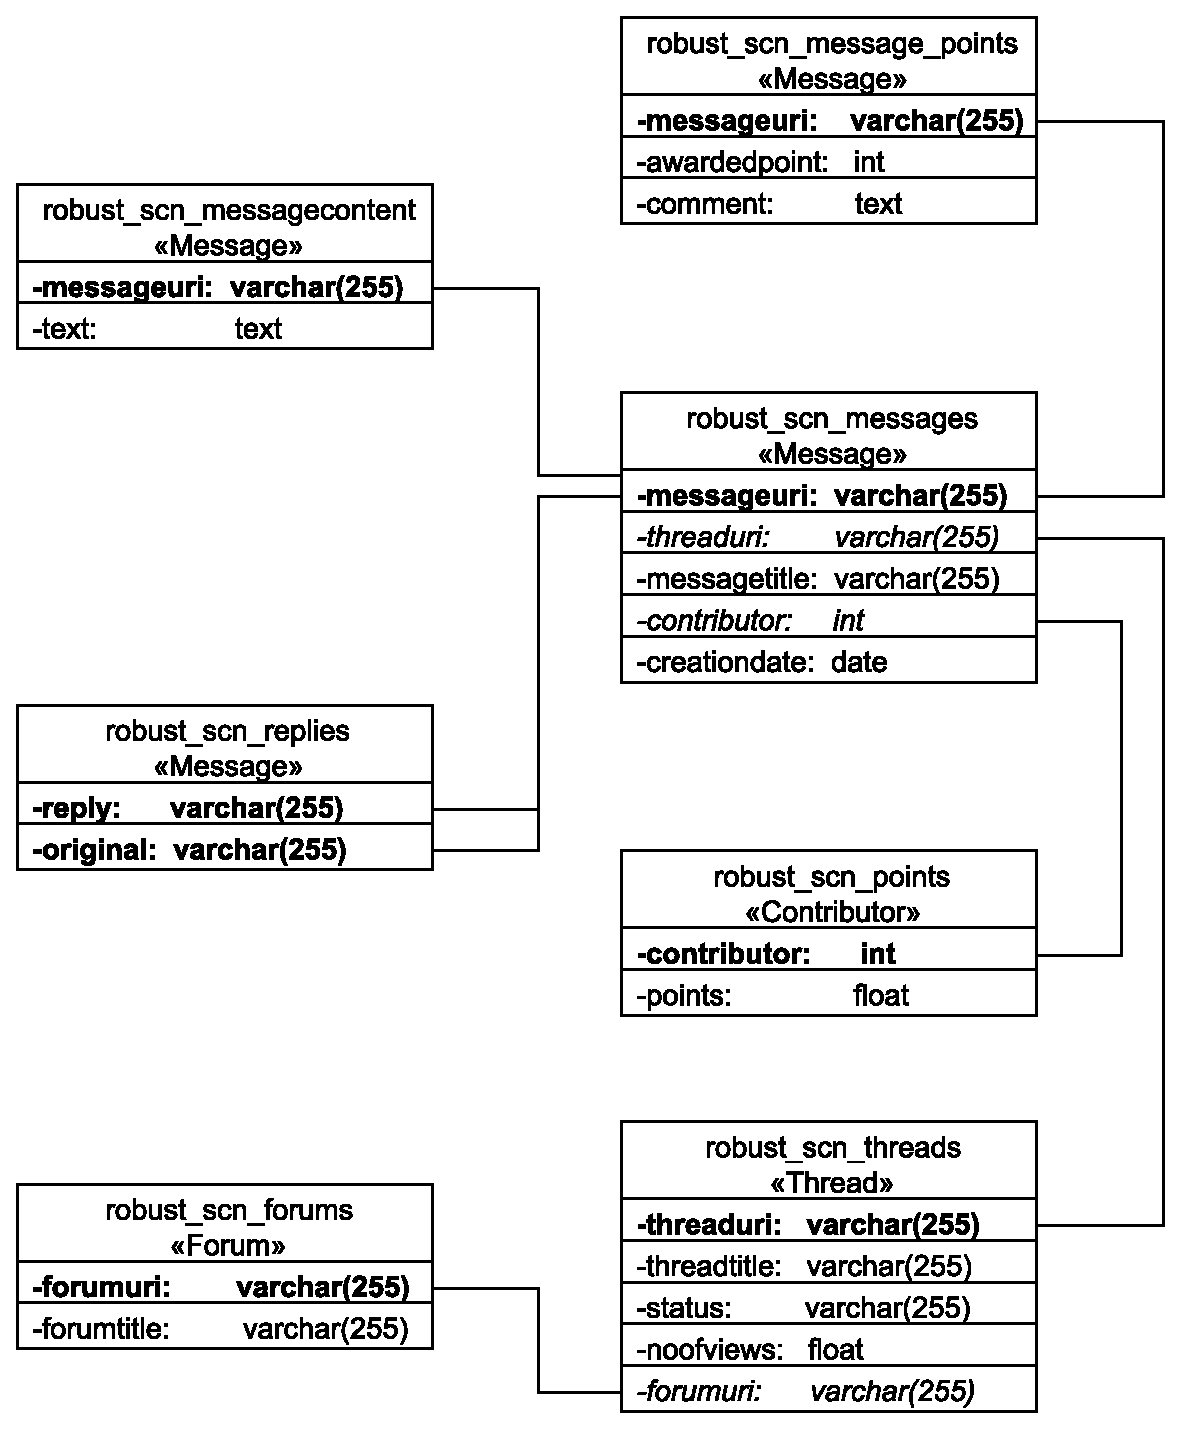
\includegraphics[scale=0.6]{05_01_relational_data_model.eps}
  \caption{The relational data model for the SAP Community Network forum.}
  \label{Figure:05_01}
\end{figure}
\fref{Figure:05_01} presents the relational data model of the SCN forum provided by SAP as a business partner use case of the ROBUST project \citep{Adrian2011}. The data model consists of four entities: the forum, contributor, thread, and message. The following is a full explanation of all fields in these entities. In addition, several important concepts based on the data model will be also defined for later used.

\textbf{Contributor.}~Defined in the \emph{robust\_scn\_points} data table, the \emph{contributor} refers to a contributor. The contributor field uniquely identifies a particular contributor. SAP does not provide the nicknames because of data privacy restraints, so each contributor will be labelled with the contributor field in the user interface. The \emph{points} field refers to the accumulated points this contributor has ever been awarded in the last twelve months and will be changed over time.

\textbf{Forum.}~Defined in the \emph{robust\_scn\_forums} data table, the forums refers to a collection of groups hierarchically organised to help contributors find their interesting discussions to participate in. For example, the SAP Business One SDK forum mainly includes something relevant to this specific discussion. The \emph{forumuri} field uniquely identifies a tuple in the table, while the \emph{forumtitle} field indicates the name of this forum. It should be noticed that forums are persistent although their content may change over time.

\textbf{Thread.}~Defined in the \emph{robust\_scn\_threads} data table, the thread refers to a series of messages concerning the same topic. The \emph{threaduri} field uniquely identifies a tuple in the table, while the \emph{threadtitle} field indicates the name of this thread. The \emph{forumuri} field defines the forum this thread belongs to. The status field indicate the current status of this thread and possible values includes `answered' and `unanswered'. The \emph{noofviews} field refers to the number of views of this thread.

\textbf{Message.}~The message refers to a written piece of information posted by a contributor, which is the building block of the SCN forum. Generally speaking, messages describes the post relationship between contributors and threads, which forms the basic activity in the SCN forum.

The main fields of messages are defined in the \emph{robust\_scn\_messages} data table. The \emph{messageuri} field uniquely identifies a tuple in the table, while the \emph{messagetitle} field indicates the name of this message. The \emph{threaduri} field defines the thread this message belongs to. The \emph{contributor} field shows the contributor of this message, which corresponds to the field with the same name in the \emph{robust\_scn\_points} data table. The \emph{creationdate} field refers to the time point when this message has been created.

The original message and reply message are defined as the \emph{original} and \emph{reply} field in the \emph{robust\_scn\_replies} data table, respectively. The latter is any message within a thread which replies to the former. Both correspond to the \emph{messageuri} field in the \emph{robust\_scn\_messages} data table. In addition, the SCN forum supports further nesting where an original message may be the reply message of another. From this point of view, each thread consists of a top-level message which is the first original message in chronological order, as well as a number of messages which directly or indirectly reply to the top-level message. The contributor who posts the top-level message is termed the \emph{original poster} of the thread and usually addresses an issue or asks a question.

Points can be awarded to contributors for each message. The \emph{robust\_scn\_message\_points} data table defines the amount of message points and the description in the \emph{awardedpoints} and \emph{comment} fields, respectively. And the \emph{messageuri} field is used to connect the field with the same name in the \emph{robust\_scn\_messages} data table. Specifically, the original poster of a thread has the right to give points to reply messages: two points for a helpful answer which can be awarded unlimited times within this thread, six points for a very helpful answer which can be awarded twice, and ten points for a solved problem which can be awarded only once. The message which has been awarded some message points is termed \emph{awarded message}. One contributor may be awarded multiple times by posting multiple useful reply messages within a thread.

The \emph{text} field in the \emph{robust\_scn\_messagecontent} data table defines the actual textual content of the message, whilst the \emph{messageuri} field is used to link to the field with the same name in the \emph{robust\_scn\_messages} data table.

\textbf{Snapshot.}~The term snapshot, which is not included in the relational data model, refers to a snapshot of a forum state during a given period of time. The \emph{start} and \emph{end} attributes will be added as the start and end timestamps, respectively. As a consequence, each forum can be divided into a set of fractions.

\subsection{The Scope of the Work} \label{sec:scope}
The scope of the forum visualisation tool is strictly limited to the visual representation of contributors, messages, and threads in the snapshot and will not take into account the following issues:
\begin{itemize}
  \item The reply network in the snapshot;
  \item The semantic of the message textual content;
  \item The network among different forums;
  \item The evolution of the forum by contrasting a series of continuous snapshots;
  \item The simulation that attempts to predict the future state of the forum.
\end{itemize}

\subsection{Tailored Data Model}
Having defined the scope of the work, it is important to note that the relational data model shown in \fref{Figure:05_01} should be tailored by removing several unused data tables as well as adding the snapshot entity. In addition, there is another reason to do so: the tailored data model should not be coupled with a particular Internet forum. Instead, a more generic data structure is needed to guarantee it still works well when the concrete data has changed.

\fref{Figure:05_02} illustrates the tailored data model in the form of the class diagram. The \emph{Snapshot} class is designed as a subclass of the \emph{Forum} class by adding the \emph{start} and \emph{end} attributes to specify a given period of time. The data collection in the snapshot is organised in a hierarchical structure. All attributes in the \emph{Contributor}, \emph{Message} and \emph{Thread} class are mapped to the fields with the same name in the \emph{robust\_scn\_points}, \emph{robust\_scn\_messages}, and \emph{robust\_scn\_threads} data tables, respectively. However, it should be noticed that two changes have been made. Firstly, the \emph{messagepoints} field in the \emph{robust\_scn\_message\_points} data table is merged into the Message class while the \emph{comment} field has been removed. Secondly, the \emph{points} attribute in the \emph{Contributor} class refers to the accumulated points this contributor has ever been awarded in the snapshot.

From a high-level view, each snapshot which inherits from a particular forum has zero or multiple threads. Each thread must belong to an instance of the \emph{Forum} class but may not be a part of any snapshot. Each message which belongs to an object of the \emph{Thread} class has only one contributor. Additionally, the \emph{AwardedMessage} class is a subclass of the \emph{Message} class in which the \emph{awardedpoints} attribute of any instance in this class must be greater than zero.

\begin{figure}[!htb]
  \centering
  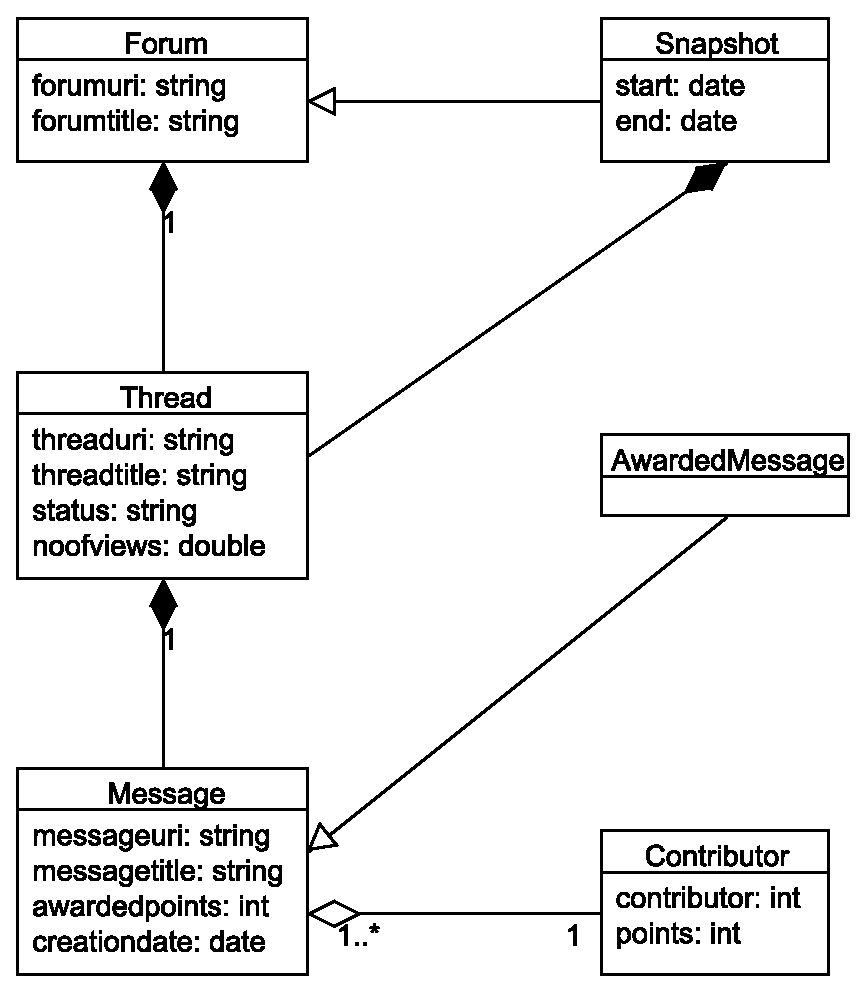
\includegraphics{05_02_class_diagram.eps}
  \caption{The class diagram for the forum visualisation tool.}
  \label{Figure:05_02}
\end{figure}

\section{Scenario} \label{sec:scenario}
This section depicts domain-specific user requirements of the forum visualisation tool in the form of the scenario  in \fref{Figure:05_03}. First of all, actors who make use of the forum visualisation tool should be identified among possible end users. Then the key scenario which details the steps of the interaction between actors and the forum visualisation tool will be clearly defined based on the risk management.

\begin{figure}[!htb]
  \centering
  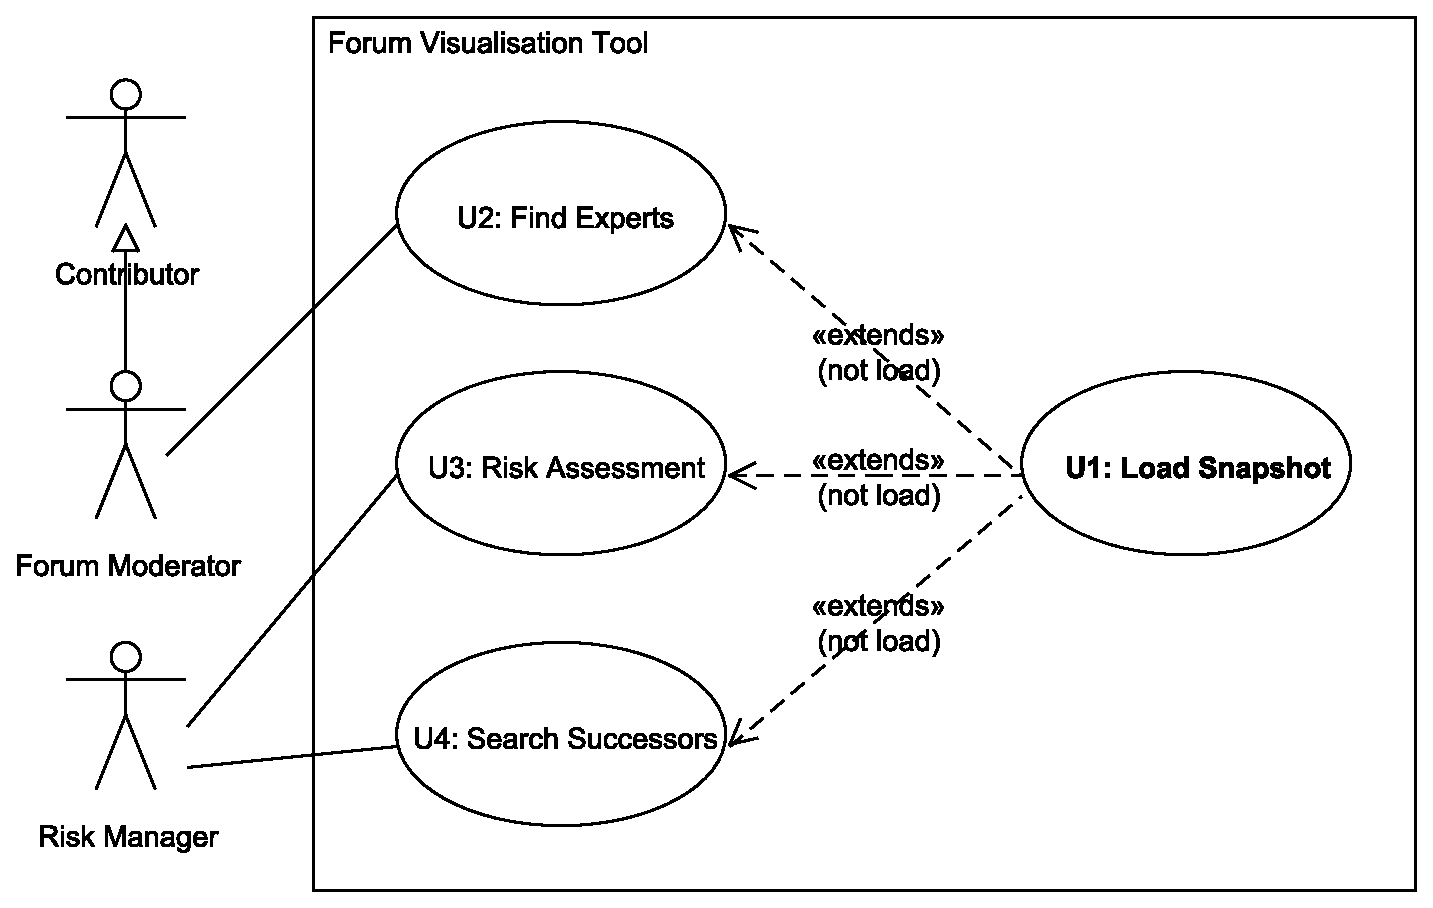
\includegraphics[scale=0.6]{05_03_use_case_diagram.eps}
  \caption{The use case diagram which includes four use cases.}
  \label{Figure:05_03}
\end{figure}

\subsection{Actors}
There are three different actors involved in the diagram: contributors, forum moderators, and risk managers. Contributors are not expected to use the forum visualisation tool directly because it is too professional for them. As a result, there is no link between contributors and any use case in the diagram. However, there is also a chance for them to make use of it in another way. The forum may share the visualisation generated by the forum visualisation tool with contributors to let them know their positions in order to encourage self-reflection.

The forum moderators are particular contributors whose primary responsibility is to promote interaction between contributors and make the forum more active. For instance, they regularly post top-level messages to add new content to the forum. The forum moderator is expected to be involved in the \emph{Find Experts} use case.

The risk managers identify any potential risk which may do harm to the forum. They are also responsible for deciding how to reduce risks if they really occurred. The risk manager is expected to be involved in the \emph{Risk Assessment} and \emph{Search Successors} use cases.

\subsection{Scenario Description}
The forum moderator intends to find out the top three experts in a given snapshot and then assign the risk manager to a task of risk assessment. Then, the risk manager receives the task and evaluates the risk by prioritise them in a reasonable order. Lastly, the risk manager completes the task by searching three potential successors who have the most similar expertise to each leaving expert, for the purpose of reducing the risk.

\subsection{Technical Description} \label{sec:tech_desc}
First of all, it is important to note that there is an implicit use case in the scenario. The \emph{Load Snapshot} use case will be only included in the \emph{Find Experts}, \emph{Risk Assessment}, and \emph{Search Successors} use cases under the condition when the snapshot data has not been loaded. Thus the snapshot data is cached in the memory once loaded from the data source.

As defined in \citep{Mcdonald2000}, an expert is a contributor who has much knowledge to answer a particular problem or moves the question toward the final resolution somehow. Apparently, this definition is twofold. In the case of the SCN forum, any contributor who has completely solved the question would be awarded ten points, while the one who has posted a helpful or very helpful answer would gain two or six points as a reward for providing useful information. Because the semantic of message content is beyond the scope of the work (see Section~\ref{sec:scope}), the awarded points of each message can be considered as the only metric to measure the quality of this message based on the assumption that the points are awarded fairly and consistently by the original poster. The more points awarded to a message, the more expertise provided from this message.

Building on the awarded points of each message, the Contributor Recognition Program (CRP)\footnote{http://www.sdn.sap.com/irj/scn/crphelp} has been developed by SCN as a level-based point system to measure the expertise of contributors. There are two distinct accumulated points for each contributor: lifetime points and annual points. The former refers to the number of points a contributor has ever been awarded since the registration date, while the latter refers to the points that a contributor has accumulated in the last twelve months on a rolling period. CRP is based on the annual points, since the SCN forum encourages contributors to contribute regularly to maintain their annual points over the rolling twelve months. Lastly, the five leading contributors in each specific forum on SCN will be displayed on the Find the Expert\footnote{http://www.sdn.sap.com/irj/scn/leadingcontributors} page.

Having discussed the strategy used in CRP, a conclusion can be drawn that the expertise of a specific contributor is proportional to the accumulated points she has ever been awarded in the snapshot for the duration of twelve months. With respect to the forum visualisation tool, an algorithm for calculating the expertise for each contributor is employed, which represents two minor differences compared with CRP. Firstly, it is possible to find experts over a flexible period of time. Secondly, the number of top experts decreases from five to three.

In this scenario, the process of the risk management has been simplified into three steps. Firstly, once the top three experts in a given snapshot have been identified by a forum moderator, a risk manager is assigned the task of the risk assessment. Secondly, this risk manager prioritises these risks in terms of the risk impact and likelihood attributes. The former refers to a possibility that the risk of experts leaving is reasonably expected to happen, while the latter represents the influence over the forum if this risk occurs. It is possible for an influential expert to walk out of the forum without any indication, which results in a big loss to the forum. Hence the priority of each risk can be defined by the combination of the likelihood and the impact. For example, an expert who has not only a strong possibility of leaving the forum but also a major impact upon her leaving should be put first. Finally, this risk manager is also in charge of seeking the treatment to reduce this risk by searching three potential successors to each expert.

\section{Use Cases} \label{sec:use_cases}
\fref{Figure:05_04} depicts the scenario in a time sequence of use cases. The key use cases are shown using red arrows, while the return values are optionally indicated using a dashed arrow. Especially, the \emph{Assign Task} use case is excluded in \fref{Figure:05_03}, because it is beyond the boundaries of the forum visualisation tool.

\begin{figure}[!htb]
  \centering
  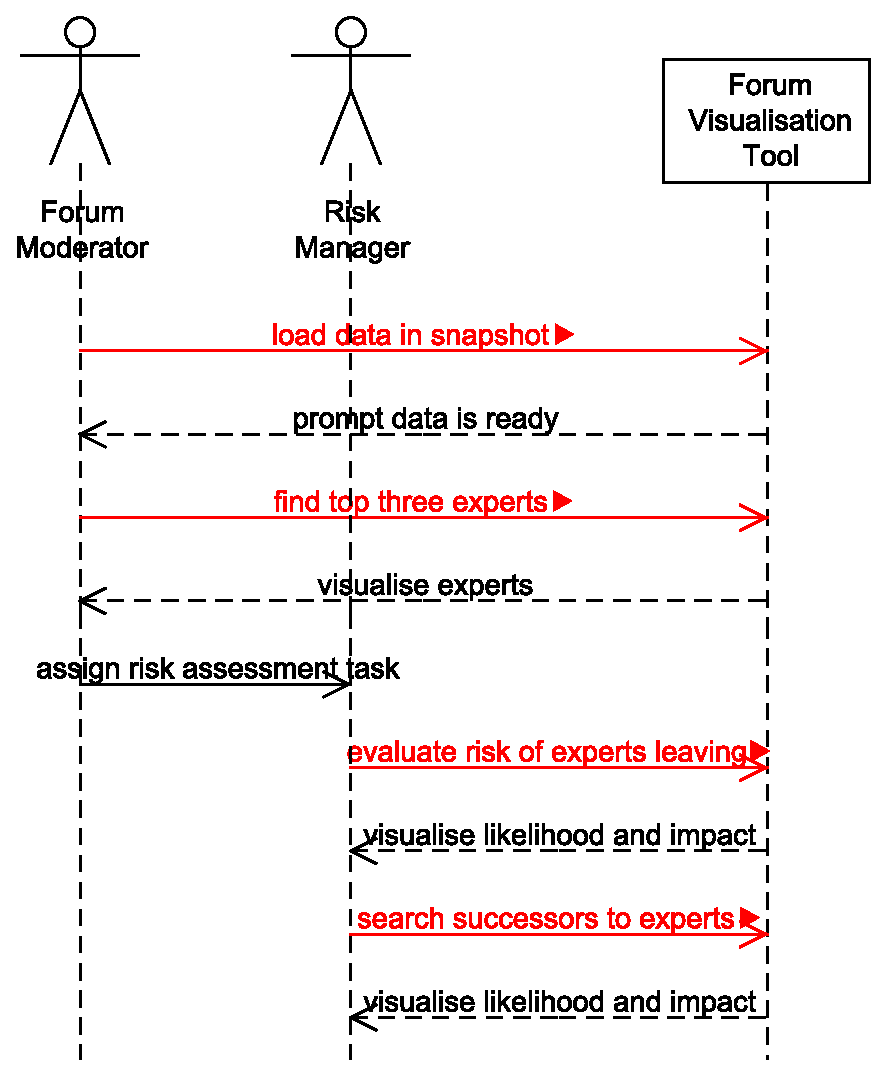
\includegraphics{05_04_sequence_diagram.eps}
  \caption{The sequence diagram depicts the scenario in a time sequence of use cases.}
  \label{Figure:05_04}
\end{figure}

\textbf{U1: Load Snapshot.}
The \emph{Load Snapshot} use case receives a period of time and a forum as input, and then returns a collection of data associated with the given snapshot.

\textbf{U2: Find Experts.}
The \emph{Find Experts} use case receives a specific snapshot as input, and then returns a graph visualisation showing the top three experts in the given snapshot under the condition that the data in the snapshot has been loaded and cached in the memory.

\textbf{U3: Risk Assessment}
The \emph{Risk Assessment} use case receives an expert and a snapshot as input, and then returns a graph visualisation showing the risk impact and likelihood under the condition that the data in the snapshot has been loaded and cached in the memory.

\textbf{U4: Search Successors}
The \emph{Search Successors} use case receives an expert and a snapshot as input, and then returns a graph visualisation showing the three potential successors to this expert under the condition that the data in the snapshot has been loaded and cached in the memory.

\section{Requirements} \label{sec:requirements}
This section summarises requirements derived from the scenario as discussed in Section~\ref{sec:scenario}. The scenario is intended to be described in an ambiguous way in order to separated it from the design and implementation of the forum visualisation tool. This section emphasises concrete requirements captured in the use cases.

\textbf{R1: General Requirements for Graph Visualisation.}
The forum visualisation tool must provide the following general requirements as infrastructure facilities for graph visualisation: navigation, interaction, built-in layout, visual properties, filtering, highlighting, clustering, satellite view, and dynamic graph. Several relevant studies have been reported in the literature. \citep{Noik1992} outlines a set of requirements which are common for graph visualisation software. Recently, a thorough list of general requirements for modern graph visualisation software has been defined in \citep{Zabiniako2009}, where the author lists more than forty concrete requirement derived from fifteen high-level requirements.

\textbf{R2: Contributor-to-Contributor Graph Visualisation.}
A contributor-to-contributor graph visualisation must be offered to present the expertise of contributors as well as the common expertise among them. This graph visualisation is the building block of the forum visualisation tool, and plays a pivot role in the \emph{Find Experts}, \emph{Risk Assessment}, and \emph{Search Successors} use cases.

First of all, this graph visualisation must provide a way for forum moderators to find the top three experts in a global perspective. Technically, contributors are expected to be rendered as nodes to represent an entity, whilst the common expertise between two contributors is displayed as edge to represent the social relationship in the graph visualisation. The expertise of contributors would be mapped to the node size. Therefore it is quite easy for forum moderators to find out the top experts by observing the largest node.

In addition, the forum visualisation tool must allow risk managers to evaluate the risk of experts leaving in terms of the risk impact and likelihood. The risk assessment is twofold. On the one hand, these two attributes are expected to be observed in the graph visualisation which gives two reasonable metric to measure the possibility that an expert may leave the forum, as well as the impact of an expert leaving on the forum. For simplicity, the design of the risk assessment is based on two basic assumptions. Firstly, the likelihood attribute is denoted by the ratio between the accumulated points which have been awarded to a specific contributor and the sum of points which have been awarded to all contributors in a given snapshot. In general, the higher the ratio, the greater risk that this expert will leave the forum. Secondly, the impact attribute indicates the percentage of the individual expertise of a specific expert. The higher the percentage, the more negative impact on the forum. On the other hand, the forum visualisation tool must provide a detailed visualisation from the perspective of each contributor in order to reveal the distribution of these two attributes over time.

Lastly, the forum visualisation must support an algorithm to divide all contributors into subgroups where all members in each subgroup has similar expertise and can be a potential successor if someone is leaving the forum.

\textbf{R3: Contributor Centric Graph Visualisation.}
The forum visualisation tool must provide a graph visualisation to allow users to explore the risk of experts leaving in terms of the risk impact and likelihood. Specifically, it is essential to offer a timeline from the start of the given snapshot to the end, as well as a time series chart to visualise the evolution of the likelihood and impact. Most importantly, an interactive graph visualisation from the experts' point of view must be established to chronologically illustrate all her behaviours with relevant threads by posting messages.

\textbf{R4: Background Thread.}
The forum visualisation should make use of a background thread to load data in snapshot. It should be avoided to execute this long-time task in the event dispatch thread, which may lead to a low responsive user interface. Added to that, the task being executed in the background thread should be cancelled before completely finish.

\section{Summary}
In this chapter the original data model provided by the SCN forum has been described with a detailed analysis of all data tables before the scope of the work is defined. Then a tailored data model is given in the form of the class diagram. Next, a scenario has been illustrated which consists of four use cases from loading snapshot data to searching successors to leaving experts. Lastly, a set of requirements has been derived from the scenario and corresponding use cases. 

%% ----------------------------------------------------------------
%% Design.tex
%% ---------------------------------------------------------------- 
\chapter{Design of the Forum Visualisation Tool} \label{Chapter:Design}

This chapter first introduces the contributor-thread graph to present how contributors post messages to threads. Then the collaborator-thread graph will be generated from the contributor-thread graph by imposing several restrictions. Next, we define the collaborative graph which is a collaborator-to-collaborator graph transformed from the collaborator-thread graph, as well as the egocentric collaborator-thread graph which is a partial graph of the collaborator-thread graph from the perspective of a centric collaborator. For each graph we not only give the clear definition but also provide the sample diagram. Lastly, we depict the user interface design details of the snapshot explorer, collaborative graph visualisation and collaborator-thread graph visualisation.

\section{Graph Design} \label{sec:graph_design}

This section first defines three types of graphs, and then presents corresponding metrics as well as visual properties. Next, the enhanced data model will be given, which involves several concepts introduced in this section.
 
\subsection{Contributor-Thread Graph} \label{sec:contributor_thread_graph}

The contributor-thread graph shows individuals' everyday behaviours in the SCN forum that contributors post messages to threads. As shown in \fref{Figure:06_01}, the message is represented by an edge that connects a contributor (circle node) and a thread (square node).

\begin{figure}[!htb]
  \centering
  \includegraphics{06_01_basic_elements_in_contributor_thread_graph}
  \caption{The basic elements in the contributor-thread graph.}
  \label{Figure:06_01}
\end{figure}

The edges are only plotted between nodes from two disjoint sets. More precisely, there is no edge between two contributors or between two threads. As a consequence, the graph:
\[G=(V, E)\]
Where \(G\) is the graph and \(E\) is a set of edges. Especially, \(V\) is a set of nodes with the restriction of a partition:
\[V=(C \cup T)\]
And every edge in \(E\) is between \(c\) to \(t\) for some \(c\) in \(C\) and \(t\) in \(T\), so that the graph is a bipartite graph:
\[G=(C, T, E)\]
The two partitions are represented by a set of contributors and a set of threads, respectively. The edges that link the nodes refer to messages and the edge weight is denoted by the \emph{awardedpoints} attributes in \fref{Figure:06_09}. Specifically, a message labelled with zero has not been awarded any point yet.

For example, consider a contributor-thread graph shown in \fref{Figure:06_02}. The graph consists of four contributors (\(C_{1}\), \(C_{2}\), \(C_{3}\), \(C_{4}\), and \(C_{5}\)), four threads (\(T_{1}\), \(T_{2}\), \(T_{3}\), \(T_{4}\), and \(T_{5}\)), and thirteen messages. The label on the edge refers to the \emph{awardedpoints} attributes of each message. Additionally, there might be multiple edges between a contributor and a thread \((C_{1} - T_{1})\) because a contributor may post several messages to a thread.

\begin{figure}[!htb]
  \centering
  \includegraphics{06_02_sample_contributor_thread_graph}
  \caption{A sample contributor-thread graph, which contains five contributors, five threads, and thirteen messages.}
  \label{Figure:06_02}
\end{figure}

In a specific thread of the contributor-thread graph, there exist a set of contributors:
\[C_{t}=(C_{1} \cup C_{2} \cup ... \cup C_{n})\]
Where \(n > 1\), \(t\) is this thread and \(C_{t}\) is the set of contributors correspond to \(t\). \(C_{1}\) to \(C_{n}\) are contributors who have ever posted at least one awarded message (see Section~\ref{sec:data_model}) to \(t\). Hence several important terms can be defined:

\begin{enumerate}
	\item Any \(c\) in \(C_{t}\) is termed the \textbf{collaborator} on thread \(t\); \\
	\item Thread \(t\) is termed \textbf{collaborative thread}; \\
	\item Any awarded message in \(E\) which connects some \(c\) in \(C_{t}\) and \(e\) in \(E\) is termed \textbf{collaborative message}, while any other awarded message in \(E\) is termed \textbf{non-collaborative message}; \\
	\item \(C_{t}\) is termed the \textbf{collaborator set} on thread \(t\); \\
	\item When \(k = 2\), the set of all \(k\)-combinations of a set \(C_{t}\) is termed \textbf{collaboration set} and denoted by \(\binom{C_{t}}{2}\). The element in this set is named \textbf{collaborative pair}, which is a pair of collaborators on thread \(t\).

\end{enumerate}

For example, consider the thread \(T_{2}\) in \fref{Figure:06_02}. The collaborator set on collaborative thread \(T_{2}\) is made up of three collaborators \(C_{1}\), \(C_{2}\), \(C_{3}\). The collaboration set consists of three collaborative pairs \((C_{1}, C_{2})\), \((C_{1}, C_{3})\), \((C_{2}, C_{3})\). Similarly, the collaborator set on T1 contains C1 and C2 while the collaboration set consists of only one collaborative pair \((C_{1}, C_{2})\). If we consider two collaboration sets as a whole, there are three unique collaborative pairs \((C_{1}, C_{2})\), \((C_{1}, C_{3})\), \((C_{2}, C_{3})\).

\subsection{Collaborator-Thread Graph}

We impose three restraints on the contributor-thread graph \(G=(C, T, E)\) to generate the collaborator-thread graph:
\[G'=(C', T', E')\]
Where \(G'\) is the graph and \(E'\) is a set of edges. \(C'\) and \(T'\) refer to the set of collaborator nodes and thread nodes, respectively.

\begin{enumerate}
	\item \(T'\) consists of any collaborative thread in \(T\); \\
	\item \(C'\) consists of any collaborator in the union of all collaborator sets; \\
	\item \(E'\) consists of any collaborative message in \(E\).
\end{enumerate}	
	
For example, the collaborator-thread graph in \fref{Figure:06_03} is generated from the contributor-thread \fref{Figure:06_02}. \(T'\) is made up of \(T_{1}\), \(T_{2}\), and \(T_{3}\) whilst \(C'\) consists of \(C_{1}\), \(C_{2}\), \(C_{3}\), and \(C_{5}\).

\begin{figure}[!htb]
  \centering
  \includegraphics{06_03_sample_collaborator_thread_graph}
  \caption{The collaborator-thread graph generated from contributor-thread graph in \fref{Figure:06_02}.}
  \label{Figure:06_03}
\end{figure}

\subsection{Egocentric Collaborator-Thread Graph}

Before defining the egocentric collaborator-thread graph, we should first introduce the concept of the distance between two nodes. In graph theory, it refers to the number of edges in a shortest path linking them. For example, the distance between \(C_{1}\) and \(T_{3}\) in \fref{Figure:06_03} is three.

The following constraints can be placed on the collaborator-thread graph \(G'=(C', T', E')\) to generate an egocentric collaborator-thread graph:
\[G'_{\alpha}=(C'_{\alpha}, T'_{\alpha}, E'_{\alpha})\]
Where \(G'_{\alpha}\) is the graph and \(\alpha\) is the centric collaborator. \(E'_{\alpha}\) is a set of edges. \(C'_{\alpha}\) and \(T'_{\alpha}\) refer to the set of collaborator nodes and thread nodes, respectively.

\begin{enumerate}
	\item \(C'_{\alpha}\) includes any collaborator of distance = 2 from \(\alpha\); \\
	\item \(T'_{\alpha}\) includes any thread of distance = 1 from \(\alpha\); \\
	\item \(E'_{\alpha}\) includes any message in \(E'\) which connects some \(c\) in \(C'_{\alpha}\) and \(t\) in \(T'_{\alpha}\).
\end{enumerate}

For example, \fref{Figure:06_04} illustrates \(C_{1}\)'s collaborator-thread graph generated from the contributor-thread in \fref{Figure:06_03}. \(T'_{C_1}\) is made up of \(T_{1}\) and \(T_{2}\) whilst \(C'_{C_1}\) consists of \(C_{1}\), \(C_{2}\), and \(C_{3}\).

\begin{figure}[!htb]
  \centering
  \includegraphics{06_04_sample_egocentric_collaborator_thread_graph}
  \caption{The egocentric collaborator-thread graph generated from collaborator-thread graph in \fref{Figure:06_03}.}
  \label{Figure:06_04}
\end{figure}

\subsection{Collaborative Graph}

The collaborative graph is a single-edge, undirected, and weighted graph, which is generated from the collaborator-thread graph. It shows an indirect relation between collaborators. In other words, one collaborator is connected to another because they have posted awarded messages to the same thread, although they may not have replied to each other.

As described in Section~\ref{sec:contributor_thread_graph}, the relation between two collaborators in the collaborator set is termed collaborative pair. Compared with the pairs that have only collaborated once, the pairs who have collaborated many of the same thread have a closer link. Therefore the weight of a collaborative pair is denoted by the number of collaborative threads it belongs to.

Given a collaborator-thread graph \(G'=(C', T', E')\), the collaborative graph:
\[G''=(V'', E''))\]
Where \(G''\) is the graph and \(E''\) is a set of edges. \(V''\) refers to the set of nodes.

\begin{enumerate}
	\item \(V''\) consists of any collaborator in \(C'\); \\
	\item \(E''\) consists of any collaborative pair in the union of all collaboration sets. The edge weight is denoted by the number of collaborative thread this collaborative pair belongs to.
\end{enumerate}

Take the collaborator-thread graph in \fref{Figure:06_03} for example. According to the definition, we should first find out all collaborators as the nodes and all collaborative pairs as the edges. As shown in \fref{Figure:06_05}, the graph is made up of four collaborators (\(C_{1}\), \(C_{2}\), \(C_{3}\), and \(C_{5}\)) as well as four edges plotted among them. The edge weight of (\(E_{12}\) is two because this collaborative pair belongs to two collaborative threads (\(T_{1}\) and \(T_{2}\)), while other edges including (\(E_{13}\), (\(E_{23}\), and (\(E_{25}\) are all weighted with one.

\begin{figure}[!htb]
  \centering
  \includegraphics{06_05_sample_collaborative_graph}
  \caption{The collaborative graph generated from the collaborator-thread graph in \fref{Figure:06_03}.}
  \label{Figure:06_05}
\end{figure}

\subsection{Metrics of Collaborative Graph} \label{sec:collaborative_graph_metrics}

This section defines several metrics of the collaborative graph, which will be mapped to diverse visual properties of the collaborative graph visualisation.

\textbf{Contribution.}~The contribution refers to the sum of points a collaborator has ever been awarded in the snapshot. As discussed in Section~\ref{sec:tech_desc}, the contribution represents the expertise of a specific contributor in the snapshot. There are four interconnected measures of contribution. The first two metrics are related to individuals while the last two metrics reflect the community nature. The sum of the first two metrics is termed individual contribution, and the sum of the last two metrics is termed community contribution. The collaborative contribution (individual) which is the accumulated points earned from all collaborative messages, and non-collaborative contribution (individual) which is the accumulated points gained from all non-collaborative messages. In contrast to the contribution which has been awarded to individuals, the sum of all collaborative contribution (individual) is named by the collaborative contribution (community), whilst the sum of all non-collaborative contribution (individual) is termed the non-collaborative contribution (community).

\textbf{Risk Attributes.}~In the \emph{Risk Assessment} use case (see U3 in Section~\ref{sec:use_cases}), the risk of experts leaving has been analysed in the aspects of the risk impact and likelihood (see R2 in Section~\ref{sec:requirements}). Having introduced four measures of the contribution, it is easy to define these two metrics. More precisely, the likelihood attribute refers to the ratio of the individual contribution to community contribution. The impact attribute is denoted by the ratio between non-collaborative contribution to contribution. \fref{Figure:06_06} presents the likelihood and impact of each contributor as well as the above-mentioned contribution metrics based on the collaborative graph shown in \fref{Figure:06_05}.

\begin{figure}[!htb]
  \centering
  \includegraphics[width=13cm]{06_06_sample_collaborative_graph_likelihood_impact}
  \caption{The contribution, likelihood, and impact metrics in the sample collaborative graph.}
  \label{Figure:06_06}
\end{figure}

\textbf{Degree Centrality.}~The degree centrality is the total number of edges connected to a particular node, which determines the relative importance of a node in the graph. This metric identifies collaborators that actively collaborate or collaborators through which flows most of the expertise. Both are critical members of the forum because their leaving may limit the exchange of expertise. However, this metric does not differentiate between quantity and quality. Take the collaborative graph in \fref{Figure:06_05} for example, the degree centrality of \(C_{2}\) is three, but it does not recognize the difference between a link to the \(C_{1}\) whose contribution is 24 points and a link to \(C_{5}\) whose contribution is only 2 points.

\textbf{Betweenness Centrality}~The betweenness centrality labels each node with a value which is the number of shortest paths that pass through it. Take the collaborative graph in \fref{Figure:06_05} for example, there are two shortest paths that pass through \(C_{2}\) (\(E_{12}\)-\(E_{25}\) and \(E_{23}\)-\(E_{25}\)), thus the betweenness centrality of \(C_{2}\) is two. Especially, this measure can be also applied to an edge that represents a collaborative pair in the collaborative graph. The edge betweenness of \(E_{25}\) in \fref{Figure:06_05} is three because there are three shortest paths pass through it \(E_{25}\), \(E_{12}\)-\(E_{25}\), and \(E_{23}\)-\(E_{25}\). \fref{Figure:06_07} presents the degree centrality and node betweenness centrality as well as the edge betweenness centrality of the collaborative graph shown in \fref{Figure:06_05}.

\begin{figure}[!htb]
  \centering
  \includegraphics[width=13cm]{06_07_sample_collaborative_graph_degree_betweenness}
  \caption{The degree centrality, node betweenness centrality, and edge betweenness centrality in the sample collaborative graph.}
  \label{Figure:06_07}
\end{figure}

Within graph theory, the bridge is a special type of edge that would divide the whole graph into several disjoint subgroups if it was removed. In the collaborative graph, consider again the edge that represents the collaborative pair, the edges with a high betweenness centrality play a vital role because they act as the bridge to connect separated subgroups. Hence, the concept of edge betweenness centrality will be used in the cluster finding algorithm which is detailed in Section~\ref{Section:WGN}.

\subsection{Weighted Girvan-Newman Algorithm} \label{Section:WGN}

The cluster finding algorithms have been widely proposed in the literature to detect subgroups. Although most of them are specifically designed for unweighted graphs, some others can be also used in weighted graphs. For example, when the edge weight is taken into account, the Weighted Girvan-Newman algorithm \citep{Newman2004} simply add an extra step of division by the weight of the corresponding edge based on the original Girvan-Newman algorithm \citep{Girvan2002}. The idea of the Weighted Girvan-Newman algorithm can be briefly described as follows:
\begin{enumerate}
	\item Calculate the edge betweenness of all edges in the graph; \\
	\item Divide each edge betweenness by the corresponding edge weight. This result is termed generalised edge betweenness; \\
	\item Remove the edge with the highest generalised edge betweenness to form a new graph. Especially, if multiple edges have the same generalised edge betweenness, remove any of them; \\
	\item Check if there exists any edge in the new graph. If yes then go to step 1, if no then end the algorithm.
\end{enumerate}

\fref{Figure:06_08} presents the detailed process of the Weighted Girvan-Newman algorithm based on the collaborative graph in \fref{Figure:06_05}.

\begin{figure}[!htb]
  \centering
  \includegraphics[width=13cm]{06_08_sample_collaborative_graph_weighted_girvan_newman_algorithm}
  \caption{The Weighted Girvan-Newman algorithm in the sample collaborative graph.}
  \label{Figure:06_08}
\end{figure}

\subsection{Visual Properties of Collaborative Graph} \label{sec:collaborative_graph_visual_props}

The visual properties play a crucial role in the node-edge diagram, which includes the node size, node colour, node opacity, node label, edge thickness, and edge colour.

\textbf{Node Size.}~In the collaborative graph, the node size represents the importance of the collaborator in the graph from three different aspects: the contribution, degree centrality, and betweenness centrality (see Section~\ref{sec:collaborative_graph_metrics}). When posting multiple awarded messages, a contributor can be awarded more than 10 points in a single thread. In this case, a contributor who gained all message points only from a single thread may be the highest in the graph. But we cannot definitely infer this contributor is the most important individual, because we should take the centrality metrics into account. For example, if the node size is mapped to the degree centrality, the node with the maximum degree has the biggest size in the graph. By default, it is mapped to the contribution of the collaborator:

\[S(v)=S_{min} + \frac{(S_{max} - S_{min}) \times P(v)}{P_{max}}\]

Where \(v\) is any node in the graph and \(S(v)\) is the node size of \(v\). \(S_{max}\) and \(S_{min}\) are the biggest and smallest node size. \(P_{max}\) is the maximum contribution in the graph and \(P(v)\) is the contribution of \(v\). For example, consider the collaborative graph in \fref{Figure:06_05}:

\[S(C_{1})=8 + \frac{50 \times 14}{22}=40 \quad \quad S(C_{2})=8 + \frac{50 \times 22}{22}=58\]
\[S(C_{3})=8 + \frac{50 \times 2}{22}=13 \quad \quad S(C_{5})=8 + \frac{50 \times 6}{22}=22\]

Where \(S_{min} = 8\) and \(S_{max} = 58\). Similarly, the node size based on other metrics:

\[S(v)=S_{min} + \frac{(S_{max} - S_{min}) \times D(v)}{D_{max}}\]
\[S(v)=S_{min} + \frac{(S_{max} - S_{min}) \times B(v)}{B_{max}}\]

Where \(D_{max}\) is the maximum degree centrality while \(B_{max}\) is the maximum betweenness centrality. \(D(v)\) and \(B(v)\) are the degree centrality and betweenness centrality of \(v\), respectively.

\textbf{Node Colour.}~The colour of each node is mapped to the risk impact attribute, which ranges from 0 to 1. Four different colours are provided to visualise this metric:

\[C(v) = \left\{\begin{array}{l l}
    RGB(255,0,0) \quad \quad 0.75 < I(v) < 1\\
    RGB(255,165,0) \quad \quad 0.5 < I(v) \leq 0.75\\
    RGB(255,255,0) \quad \quad 0.25 < I(v) \leq 0.5\\
    RGB(0,255,0) \quad \quad 0 < I(v) \leq 0.25
  \end{array} \right.
\]

Where \(v\) is any node in the graph and \(C(v)\) is the node colour of \(v\) in the form of RGB code. \(I(v)\) is the risk impact of \(v\). For example, consider the collaborative graph in \fref{Figure:06_05}:

\[C(C_{1})=RGB(255,255,0) \quad \quad C(C_{2})=RGB(0,255,0)\]
\[C(C_{3})=RGB(0,255,0) \quad \quad C(C_{5})=RGB(0,255,0)\]

\textbf{Node Opacity.}~The opacity of each node is mapped to the risk likelihood attribute, which also ranges from 0 to 1. With the purpose of ensuring each node is visible, the minimum opacity is expected to be taken into account:

\[O(v)=O_{min} + \frac{(o_{max} - O_{min}) \times L(v)}{O_{max}}\]

Where \(v\) is any node in the graph and \(O(v)\) is the node opacity of \(v\). \(O_{max}\) and \(O_{min}\) are the highest and lowest node opacity. \(L(v)\) is the risk likelihood of \(v\). For example, consider the collaborative graph in \fref{Figure:06_05}:

\[O(C_{1})=0.5 + \frac{0.5 \times 0.44}{1}=0.77 \quad \quad O(C_{2})=0.5 + \frac{0.5 \times 0.41}{1}=0.71\]
\[O(C_{3})=0.5 + \frac{0.5 \times 0.04}{1}=0.52 \quad \quad O(C_{5})=0.5 + \frac{0.5 \times 0.11}{1}=0.56\]

Where \(O_{max} = 1\) and \(O_{min} = 0.5\).

\textbf{Node Label.}~The label of nodes displays the \emph{contributor} attribute of the \emph{Contributor} class (see Section~\ref{sec:data_model}). The label visibility is determined by the node size, which is configurable in the visual properties panel in the graph options window (see Section~\ref{sec:collaborative_graph_options_window}).

\textbf{Edge Thickness.}~The thickness of edges indicates to what extend a collaborator pair has the similar expertise, or how tightly they connect with. By default, it is mapped to the edge weight:

\[T(e)=T_{min} + \frac{(T_{max} - T_{min}) \times W(e)}{W_{max}}\]

Where \(e\) is any edge in the graph and \(T(e)\) is the edge thickness of \(e\). \(T_{max}\) and \(T_{min}\) are the biggest and smallest edge thickness. \(W_{max}\) is the maximum edge weight in the graph and \(W(e)\) is the edge weight of \(e\). For example, consider the graph in \fref{Figure:06_05}:

\[T(E_{12})=1 + \frac{4 \times 2}{2}=5 \quad \quad T(E_{13})=1 + \frac{4 \times 1}{2}=3\]
\[T(E_{23})=1 + \frac{4 \times 1}{2}=3 \quad \quad T(E_{25})=1 + \frac{4 \times 1}{2}=3\]

Where \(T_{max} = 5\) and \(T_{min} = 1\).

\textbf{Edge Colour.}~The colour of nodes is preserved for the use of highlighting and clustering. By default, the node colour is light grey.

\subsection{Visual Properties of Collaborator-Thread Graph}
Similar to the collaborative network, there are two visual properties in the collaborator-thread graph.

\textbf{Node Icon.}~Since there are two distinct nodes in the graph, two icons is used to distinguish the collaborator node and thread node.

\textbf{Edge Thickness.}~The edge thickness is mapped to the awarded points of the message:

\[T(e) = \left\{\begin{array}{l l}
    1 \quad \quad P(e) = 2\\
    2 \quad \quad P(e) = 6\\
    4 \quad \quad P(e) = 10
  \end{array} \right.
\]

Where \(e\) is any edge in the graph and \(T(e)\) is the edge thickness of \(e\). \(P(e)\) is the awarded points of \(e\).

\subsection{Enhanced Data Model}

\fref{Figure:06_09} shows the enhanced class diagram based on the tailored data model (see \fref{Figure:05_02}) by adding several concepts introduced in Section~\ref{sec:contributor_thread_graph}.
 
In the centre of the diagram, the \emph{CollaborativeThread} class is a subclass of the \emph{Thread} class, which contains at least one instance of the \emph{CollaborativePair} class. For each collaborative pair, it contains exactly two distinct instance of the Collaborator class. In addition, there is an attribute \emph{amount} to indicate the number of collaborative thread it belongs to. The constraints on the \emph{Collaborator} class are that any instance in this class is also an instance of the Contributor class and must belong to at least one collaborative pair.

Now we can realise the collaborator-thread graph as well as the collaborative graph more clearly with the help of \fref{Figure:06_09}. The collaborator node and thread node of the collaborator-thread graph are actually the \emph{Collaborator} class and the \emph{CollaborativeThread} class, respectively. The edges of the collaborator-thread graph consist of any instance in the \emph{AwardedMessage} class which is posted by a collaborator. The edge weight is the \emph{awardedpoints} attribute. Similarly, the node and edge of the collaborative graph refer to the \emph{Collaborator} and \emph{CollaborativePair} class, respectively. The edge weight is the \emph{amount} attribute.

\begin{figure}[!htb]
  \centering
  \includegraphics[width=13cm]{06_09_enhanced_class_diagram}
  \caption{The enhanced data model by adding basic concepts for the forum visualisation tool.}
  \label{Figure:06_09}
\end{figure}

\fref{Figure:06_10} shows a sample object diagram generated from the contributor-thread graph in \fref{Figure:06_02}. The instances in grey are excluded from the collaborator-thread graph. The object t4 in the bottom left of the diagram is not a collaborative thread because it does not contain any object of the \emph{CollaborativePair} class. The object m4, m5, and m9 are not objects of the \emph{AwardedMessage} class because they have not been awarded any point. Especially, the object m12 in the bottom centre of the diagram is awarded ten points. But it is posted by c4 who is not an object of the \emph{Collaborator} class. The object c4 is not an object of the \emph{Collaborator} class because it does not belong to any instance of the \emph{CollaborativePair} class. In the collaborative graph, the object cp1 is an edge between two objects c1 and c2 with the weight two because cp1 belongs to two distinct threads t1 and t2.

\begin{figure}[!htb]
  \centering
  \includegraphics[width=13cm]{06_10_sample_object_diagram}
  \caption{The sample object diagram generated from the contributor-thread graph in \fref{Figure:06_02}.}
  \label{Figure:06_10}
\end{figure}

\section{User Interface Design}

In Section~\ref{sec:requirements}, R2 and R3 have imposed two requirements in the the collaborative graph and egocentric collaborator-thread graph, respectively. Section~\ref{sec:graph_design} have already defined these two graphs as well as their metrics and visual properties.
This section describes the user interface design of the corresponding graph visualisations. Added to that, the snapshot explorer will be also depicted.

\subsection{Snapshot Explorer}

The snapshot is not explicitly mentioned in the use case scenario discussed in Section~\ref{sec:requirements}. However it is still an indispensable component in the forum visualisation tool for two reasons. Firstly, the condition panel provides the user interface to collect the input of the \emph{Load Snapshot} use case (see U1 in Section~\ref{sec:use_cases}). Secondly, the tree view and properties window allow end users to browse the snapshot data in the traditional hierarchical structure, while the properties window displays detailed information of items in the tree view. The former has a mutual link with the main window of the collaborator-thread graph. The latter will be invoked by the main window of both collaborative graph and collaborator-thread graph. \fref{Figure:06_11} shows the main window of the snapshot explorer which consists of the conditions panel and tree view.

\begin{figure}[!htb]
  \centering
  \includegraphics[width=8cm]{06_11_snapshot_explorer_main_window}
  \caption{The main window of the snapshot explorer.}
  \label{Figure:06_11}
\end{figure}

\subsubsection{Conditions Panel}

As mentioned in the previous chapter, a snapshot is uniquely identified by the forum and a given period of time. In the conditions panel, the end users choose a forum in the drop-down list, then select the year, month, and duration to calculate the \emph{start} and \emph{end} attributes in the \emph{Snapshot} class. When clicking the Load button, a long-running cancellable task will be established in a background thread without blocking the user interface. Meanwhile, the Load button is set to disabled to guarantee there is only one task running at a time. Once the data has been loaded from the data source, the new snapshot data will be added into the tree view, and the Load button is set to enable again. In addition, the collaborative graph of this snapshot will be automatically opened in a new window.

\subsubsection{Tree View}
The tree view provides a tri-level hierarchical structure to display the snapshot data. The top level nodes represent an object of the \emph{Snapshot} class, while the second level nodes and the leaf node refer to an instance of the \emph{Thread} and \emph{Message} class, respectively. When double-clicking a particular node, the detailed information will be displayed in the properties window.

\subsubsection{Properties Window}
The properties window simply makes use of the key-value pair to list all attributes of an entity defined in the data model. \fref{Figure:06_12} presents the properties window of an object of the \emph{Thread} class.

\begin{figure}[!htb]
  \centering
  \includegraphics[width=8cm]{06_12_snapshot_explorer_properties_window}
  \caption{The properties window of the snapshot explorer.}
  \label{Figure:06_12}
\end{figure}

\subsection{Collaborative Graph Visualisation}
In this section, the user interface design of the collaborative graph visualisation will be depicted which including the main window (Section~\ref{sec:collaborative_graph_main_window}), dynamic filters window (Section~\ref{sec:collaborative_graph_filters_window}), and graph options window (Section~\ref{sec:collaborative_graph_options_window}). Additionally, the highlighting mechanism (Section~\ref{sec:collaborative_graph_highlighting}) which plays an important role in both main window and graph options window will be described in more details.

\subsubsection{Main Window} \label{sec:collaborative_graph_main_window}
\fref{Figure:06_13} presents the main window of the collaborative graph, which consists of the master view, satellite view and toolbar. The master view is the main part of the visualisation, while the satellite view on the whole or large part of the graph contains a lens shape that shows the boundaries of the visible part of the graph in the master view. The tool bar provides commonly used functionalities. The master view of the collaborative graph provides several dynamic functionalities and most of them take place via a mouse:

\begin{enumerate}
	\item Scale the whole graph with the scroll wheel or with the `Zoom In' or `Zoom Out' buttons in the toolbar; \\
	\item Fit to view by clicking the `Fit to View' button in the toolbar when the master view is too big to have an overview or too small to see details; \\
	\item Pan the whole graph by dragging the mouse in the move mode, or move around a set of nodes after selecting them by clicking on them or dragging a rectangle around them in the select mode. Add to that, multiple nodes can be also picked by holding the shift key. Two modes can be switched by clicking the `Select' or `Move' toggle buttons in the toolbar; \\
	\item Show or hide the satellite view by clicking the `Satellite' button in the toolbar; \\
	\item Show detailed information in tooltip when hovering over nodes or edges. For nodes, the information includes the \emph{contributor} and \emph{points} attributes of the \emph{Contributor} class, as well as graph metrics (e.g. degree centrality) on the fly. For edges, the information includes the \emph{amount} attribute of the \emph{CollaborativePair} class; \\
  \item Show detailed information in the properties window (see \fref{Figure:06_12}) in the context menu of nodes or edges; \\
	\item Link to the collaborator-thread graph when selecting the corresponding menu item in the context menu of nodes.
\end{enumerate}

\begin{figure}[!htb]
  \centering
  \includegraphics[width=13cm]{06_13_collaborative_graph_main_window}
  \caption{The main window of the collaborative graph.}
  \label{Figure:06_13}
\end{figure}

Based on the same model, the above interactions affect the master view as well as the lens shape in the satellite view. In addition, the visual properties in Section~\ref{sec:collaborative_graph_visual_props} are applied to both views.

\subsubsection{Highlighting} \label{sec:collaborative_graph_highlighting}

It is common to provide highlighting mechanism in the graph visualisation. Vizster \citep{Heer2005a} makes use of highlighting to annotate all friends of a specific user within a social network. By contrast, Invenio \citep{Singh2007} utilises the highlighting feature to mark different node sets in a multi-modal graph. In the collaborative graph visualisation, highlighting plays an important role in two scenarios. Firstly, when a set of nodes has been picked in the select mode, all picked nodes will be rendered in yellow. Their neighbour nodes are expected to be highlighted in red, as well as the edges that are plotted between any node in the picked node set and neighbour nodes. This feature is particularly useful in a large-scale graph as shown in \fref{Figure:06_14}, which clearly indicates all neighbour node of a set of picked nodes. Secondly, when cluster finding feature is on, each subgroup will be highlighted with a random colour which will be detailed described in the following section.

\begin{figure}[!htb]
  \centering
  \includegraphics[width=13cm]{06_14_highlighting_neighbour_nodes}
  \caption{The highlighting mechanism is used to mark neighbour nodes}
  \label{Figure:06_14}
\end{figure}

\subsubsection{Dynamic Filters Window} \label{sec:collaborative_graph_filters_window}

The filtering mechanism provides a way to remove a set of nodes and/or edges under a given set of conditions from the dual-view of the collaborative graph visualisation. As shown in \fref{Figure:06_15}, there are two panels in the dynamic filters window: node filters panel and edge filters panel.

The node filters panel consists of three metrics: contribution, degree centrality, and betweenness centrality (see Section~\ref{sec:collaborative_graph_metrics}). For each metric, a slider from zero to maximum is provided to adjust the threshold value which is displayed in the red label above each slider. When dragging the slider knob, the corresponding threshold value is also changed to remove all elements whose metric is less than the threshold value from the dual-view. For example, if the threshold value of the contribution slider is set to 100. That means any nodes whose contribution is less than 100 will be filtered out from dual-view of the collaborative graph visualisation. Moreover, if the threshold value of the contribution slider reaches the maximum, only the node with the highest contribution appears in the dual-view. Similarly, the edge filters panel is made up of the number of the collaborative thread, which is also the edge weight. Additionally, multiple aforementioned metrics can be combined to form a compound condition.

\begin{figure}[!htb]
  \centering
  \includegraphics[width=8cm]{06_15_collaborative_graph_dynamic_filters_window}
  \caption{The dynamic filter window of the collaborative graph visualisation.}
  \label{Figure:06_15}
\end{figure}

\subsubsection{Graph Options Window} \label{sec:collaborative_graph_options_window}
\fref{Figure:06_16} presents the graph options window of the collaborative graph visualisation, which can be divided into two sub-components: the cluster finding panel and the visual properties panel.

\begin{figure}[!htb]
  \centering
  \includegraphics[width=8cm]{06_16_collaborative_graph_visualisation_graph_options_window}
  \caption{The graph options window of collaborative graph visualisation.}
  \label{Figure:06_16}
\end{figure}

\textbf{Cluster Finding Panel.}~The layout algorithm is in charge of calculating the coordinate of each node. The global layout drop-down list provides a way for end users to switch the global layout displayed in both the master view and satellite view. By default, the global layout is set to Fruchterman-Reingo \citep{Fruchterman1991} since two collaborators connected with an edge that has a higher weight will be plotted much closer, in order to indicate they have more similar knowledge.

The enable cluster finding checkbox acts as an on-off switch to start and stop the clustering mechanism. When this checkbox has been selected, the edges removed slider is set to enable. The value of this slider is mapped to a threshold which determines the number of iteration in the Weighted Girvan-Newman algorithm discussed in Section~\ref{Section:WGN}. For each subgroup in the new graph generated by the algorithm, a set of random colours is expected to highlight different subgroups so that all nodes in the same group will be rendered the same colour.

Additionally, the group cluster drop-down list provides an option for end users to establish a sub-layout for each subgroup in order to gather all nodes in the same subgroup around a small region. When this drop-down list has been selected, the cluster sub-layout drop-down list can be used to change the sub-layout of all subgroups, while the sub-layout dimension drop-down list determines the size of the small region which contains all elements of the subgroup.

\textbf{Visual Properties Panel.}~The visual properties panel provides two features to configure the node label as well as the node size. The show node labels slider allows end users to input a threshold value to make any node whose node size is greater than the threshold visible. The node size is mapped to drop-down list can be used to change the metric which is mapped to the node size. Once the option of this list has been change, the master and satellite view will be immediately refreshed to display the new view.

\subsection{Collaborator-Thread Graph Visualisation}
In this section, the user interface design of the collaborator-thread graph visualisation will be depicted which including the main window (\ref{sec:c_t_graph_main_window}) and temporal chart window (\ref{sec:c_t_graph_temporal_chart_window}).

\subsubsection{Main Window} \label{sec:c_t_graph_main_window}
\fref{Figure:06_17} presents the main window of the collaborator-thread graph visualisation, which is much the same the main window of the collaborative graph visualisation.

\begin{figure}[!htb]
  \centering
  \includegraphics[width=13cm]{06_17_collaborator_thread_graph_visualisation_main_window}
  \caption{The main window of collaborator-thread graph visualisation.}
  \label{Figure:06_17}
\end{figure}

\subsubsection{Temporal Chart Window} \label{sec:c_t_graph_temporal_chart_window}
The collaborator-thread graph visualisation provides time-dependant functionalities for the risk manager to see and compare the changes over time including the risk likelihood and impact. As shown in \fref{Figure:06_18}, the temporal chart window is made up of three major components: the bar chart, the timeline slider, and the metric drop-down list.

\begin{figure}[!htb]
  \centering
  \includegraphics[width=13cm]{06_18_collaborator_thread_graph_visualisation_temporal_chart_window}
  \caption{The temporal chart window of collaborator-thread graph visualisation.}
  \label{Figure:06_18}
\end{figure}

Users are allowed to use the timeline slider to navigate through different time points by dragging the slider knob to see the evolution of the snapshot. Above the timeline slider, a bar chart shows how risk likelihood or impact changes over time, which enables users to see several important metrics during navigations. The metric drop-down list allows users to observe different metrics in the bar chart.

\section{Summary}
This chapter first defines two types of graphs: the collaborative graph and egocentric collaborator-thread graph. Then the graph metrics and corresponding visual properties have been added into the collaborative graph. Lastly, the user interface design of three major components in the forum visualisation tool have been described.

%% ----------------------------------------------------------------
%% Prototype.tex
%% ---------------------------------------------------------------- 
\chapter{Prototype of the Forum Visualisation Tool} \label{Chapter:Prototype}

This chapter outlines the specification of \emph{RiskVis}, which is a prototype of the forum visualisation tool. This specification is not intended to be exhaustive and will only focus on the architecture as well as several major modules.

\section{Architecture}

\fref{Figure:07_01} illustrates the high-level architecture of \emph{RiskVis}, which is a standalone desktop application powered by Java Desktop Technologies (Java Swing and Java 2D). It also exploits a host of third party libraries which are rendered in grey in the diagram to execute specific tasks such as the database connection and graph visualisation. Additionally, the database in the left of the diagram is based on PostgreSQL, which contains the relational data model described in Section~\ref{sec:data_model}. Furthermore, the NetBeans Platform is employed as the framework so that it is possible to develop a modular and loosely coupled application that can be easily extended in the future.

\begin{figure}[!htb]
  \centering
  \includegraphics[width=13cm]{07_01_riskvis_architecture}
  \caption{The architecture diagram of \emph{RiskVis}. Rectangles with module label refer to NetBeans modules. Dash arrows with use label refer to dependency between two modules.}
  \label{Figure:07_01}
\end{figure}

\section{NetBeans Platform}

The NetBeans Platform is a generic framework for developing Java Swing applications. \emph{RiskVis} makes use of it as the execution environment for two reasons. Firstly, it provides a complete framework which contains a number of infrastructure facilities ranged from a simple menu bar to a complicated window system, as well as a rich set of advanced Java Swing components (the explorer and properties sheet). As a consequence, more effort can be concentrated on the graph visualisation. Secondly, it also offers a solution to organise the whole application into separated modules. More precisely, a specific module is allowed to call Application Programming Interfaces (APIs) provided by other modules if and only if this caller module has explicitly defined dependencies upon those callee modules. In \fref{Figure:07_01}, the dashed arrows with the use label refer to the dependency between two modules. This section introduces five most relevant NetBeans modules to \emph{RiskVis}, which are outside the application boundary.

\subsection{Lookup API}

The Lookup API provides a way to use the dependency injection so that a module can initialise an object defined in another module without explicitly building dependency between them. This feature will be used in the snapshot explorer module.

\subsection{Window System API}

The Window System API provides a Multiple Document Interface (MDI), which contains functionality such as maximise/minimise, dock/undock, and drag-and-drop of windows. As the building block of \emph{RiskVis}, the snapshot explorer and graph visualisation discussed in the previous chapter will be managed under this window system. \fref{Figure:07_02} presents four windows being displayed simultaneously.

\subsection{Progress API}

The Progress API enables developers to use the progress bar in the bottom right of \fref{Figure:07_02}, to indicate the current progress when executing long-time tasks. This feature will be used in the snapshot explorer module.

\subsection{Explorer \& Properties Sheet API}

The Explorer \& Property Sheet API provides two advanced Java Swing components for displaying data models. The explorer in the left of \fref{Figure:07_02} allows end users to browse hierarchical data in the tree view, whilst the properties sheet in the right of \fref{Figure:07_02} displays the detailed information about an item in the tree view. This feature will be used in the snapshot explorer and graph visualisation module, which efficiently present objects defined in the enhanced data model (see \fref{Figure:06_09}).

\begin{figure}[!htb]
  \centering
  \includegraphics[width=14cm]{07_02_riskvis_screenshot}
  \caption{The screenshot presents several major feature of \emph{RiskVis} powered by NetBeans Platform, including multiple windows, progress bar in the bottom right, explorer window in the left, the properties sheet window in the right, and the global options dialogue in the centre.}
  \label{Figure:07_02}
\end{figure}

\subsection{Options and Dialogue SPI}
The Options and Dialogue SPI provides a way to integrate with the global options window in the centre of \fref{Figure:07_02} so that end users can customise the application. This feature will be used in the SCN Data Implementation module.

\section{RiskVis Module Description} \label{sec:riskvis_module_desc}

\emph{RiskVis} is made up of seven modules: the Snapshot Explorer, Graph Visualisation, SCN Data API, SCN Data Implementation, JUNG, JFreeChart, and PostgreSQL JDBC Connector. The last three modules are wrapper library modules that contain no code but the corresponding libraries: the PostgreSQL driver to connect to the SCN Forum database, the JUNG library as the graph visualisation framework discussed in Section~\ref{sec:evaluation_vis_framework}, and the chart library to draw temporal bar charts in the collaborator-thread graph visualisation (see \fref{Figure:06_18}), respectively. The section presents the other four modules in more technical details.

\subsection{SCN Data API}

As illustrated in \fref{Figure:07_03}, the SCN Data API module implements the enhanced data model (see \fref{Figure:06_09}) in the entity package. It also defines generic data access APIs in the \emph{SnapshotService} interface to get forums, threads, and messages from the data source in the form of the Java interface.

\begin{figure}[!htb]
  \centering
  \includegraphics[width=13cm]{07_03_scn_data_class_diagram}
  \caption{The class diagram including SCN Data API module and SCN Data Implementation module.}
  \label{Figure:07_03}
\end{figure}

\subsection{SCN Data Implementation}

\fref{Figure:07_03} also shows the detailed structure of the SCN Data Implementation module, which consists of the Data Access Object (DAO) package and default package. The former is designed for accessing database as a set of low-level data manipulation classes. The latter implements the \emph{SnapshotService} interface defined in the SCN Data API module by using the DAO package. Additionally, this module also includes the \emph{DBConnection} class which provides a user interface for end users to configure the database connection parameters such as the database URL, username, and password. With the aid of the Options and Dialogue SPI module, this feature has been integrated into the global options dialogue.

\subsection{Snapshot Explorer}

As the starting point of \emph{RiskVis}, the snapshot explorer module includes the condition panel (see \fref{Figure:06_11}) which allows end users to load data in any user-specified snapshot. The Lookup API is used to get an instance of the \emph{SnapshotService} interface defined in the SCN Data API module, although there is no dependency upon the SCN data Implementation module that has really provided an implementation (the \emph{SnapshotServiceImpl} class) of the interface. The benefit of this loosely coupled strategy is that any other SCN Data implementation can easily take over without any modification to the modules that use the SCN data.

As discussed in Section~\ref{sec:requirements}, the load action will be executed in the background thread with conveying the progress of the task powered by the Progress API. In this way, end users are allowed to interact with an existing snapshot when waiting for data being loaded. Once the data has been successfully loaded from the database, the new hierarchical data in the form of snapshot-thread-message is expected to be added into the tree view. Meanwhile, the collaborative graph visualisation will be automatically opened by the window system.

Additionally, it is important to note that the snapshot explorer window in this module is considered as a singleton component under the management of the window system.

\subsection{Graph Visualisation}

The graph visualisation module is the most important module of the application, which is made up of three packages: the collaborative graph visualisation, collaborator-thread graph visualisation, and utility package. \fref{Figure:07_04} presents the simple class diagram of this module, which will not be specified down to the smallest detail but from the high-level perspective.

The collaborative graph visualisation package consists of three visual components: the \emph{CollaborativeTopComponent}, \emph{CollaborativeFiltersComponent}, and \emph{CollaborativeOptionsTopComponent} class, which represent the main window (Section~\ref{sec:collaborative_graph_main_window}), dynamic filters window (Section~\ref{sec:collaborative_graph_filters_window}), and graph options window (Section~\ref{sec:collaborative_graph_options_window}), respectively. Similarly, the collaborator-thread graph visualisation consists of two visual components: the \emph{CollaboratorTopComponent}, and \emph{CollaboratorTemporalTopComponent}, which refer to the main window (\ref{sec:c_t_graph_main_window}) and temporal chart window (\ref{sec:c_t_graph_temporal_chart_window}), respectively.

The utility package provides infrastructure facilities to both graph visualisations. For example, the \emph{ClusterUtil} class makes use of the \emph{WeightedGirvanNewmanAlgorithm} class to encapsulate the cluster finding features described in Section~\ref{sec:collaborative_graph_options_window}. The \emph{GraphUtil} class calculates widely-used metrics such as degree centrality, betweenness centrality, and so forth. The \emph{PopupGraphMousePlugin} class allows end users to open the context menu when right clicking a specific element in the graph visualisation.

\begin{figure}[!htb]
  \centering
  \includegraphics[width=13cm]{07_04_graph_visualisation_class_diagram}
  \caption{The simple class diagram of the graph visualisation module.}
  \label{Figure:07_04}
\end{figure}

\section{Summary}

This chapter briefly summarises the implementation details of \emph{RiskVis} from a modular point of view. All functionalities defined in the previous chapter have been encapsulated within separate modules running in the NetBeans Platform. After an introduction of the application architecture, both the modules provided by NetBeans and those module included in \emph{RiskVis} have been described with class diagrams.

%% ----------------------------------------------------------------
%% Evaluation.tex
%% ---------------------------------------------------------------- 
\chapter{Evaluation of the Forum Visualisation Tool} \label{Chapter:Evaluation}

This chapter begins with the purpose of the evaluation of the forum visualisation tool which has been implemented in the previous chapter by pinpointing what and why to evaluate. The participants will be then depicted to clarify who will do evaluation. The method of evaluation is further defined to answer the question how to evaluate. Lastly, the results of the evaluation will be presented and discussed.

\section{Evaluation Goals}
Before the evaluation has been conducted, the goals of the evaluation should be clarified, which have significant impact upon the methods to be chosen. There are two goals in the evaluation. Firstly, a set of problems participants have encountered during the evaluation will be listed and analysed, in order to learn which specific functionality is not good. Secondly, participants are allowed to make comments about the forum visualisation tool such as rating existing features with respect of the utility of the tool, or imposing new requirements. Both encountered problems and further comments will be used to enhance the forum visualisation tool in the next iteration. In summary, the primary purpose of the evaluation is to assess to what extent the tool can be used to complete a set of tasks without external aids.

\section{Evaluation Participants}
The participants of the evaluation can be divided into two different groups. The first group consists of MSc students who undertake their dissertations with the ROBUST project. Participants in the second group are on the staff of the IT-Innovation Centre as well as the project members. All participants have prior knowledge about the SCN Forum relational data model as well as the context of the forum visualisation tool. However, the student group lacks the expertise required for understanding a number of domain-specific requirements in the context of the forum visualisation tool.

\section{Evaluation Method}
\citep{Nielsen1993} suggests that thinking-aloud method is suitable for those evaluations whose main goal is to ``help improve the user interface as part of an iterative design process''. The think-aloud method, first introduced by \citep{Lewis1982a}, refers to a usability engineering method in which the participants are required to articulate their observations, intentions, feelings, and thoughts. \citep{Nielsen1994} reveals that about 30\% of usability problems have been found when there is only a single participant involved, whilst about 80\% of the problems had been found when the number of participants increases to five.
As a result, a face-to-face interview with the help of the thinking-aloud method is chosen as the approach to evaluation of the forum visualisation tool, which involves two participants in the student group as well as two experts in the staff group. The interview has been organised in the following steps: preparation, thinking-aloud task, and debriefing.

First of all, the interview has taken place in the meeting room of the IT Innovation Centre and each interview is expected to last about 40 minutes. The computer system has also been provided by the IT Innovation Centre, in which the distribution ZIP files of \emph{RiskVis} as well as the SCN forum powered by PostgreSQL database have been correctly installed and configured before the interview.

In addition, a copy of the get started guide (see Appendix~\ref{Chapter:AppendixA}) which thoroughly details the instructions of four thinking-aloud tasks has been printed out. Also, the address of an online questionnaire (see Appendix~\ref{Chapter:AppendixB}) has been sent to the participants.

Before asking the participants to do tasks, a brief introduction of the goals of the interview as well as the thinking-aloud method will be given. Then the tasks defined in the get started guide will be described in more details. The participants are expected to execute the tasks one by one and verbalise the observations and thoughts, whether the output fulfils their expectations or not. 
After the interview, the participants are asked to fill in an online questionnaire which contains a consent form, some prior knowledge questions, a list of encountered usability problems, and any further comment about the tool.

\section{Evaluation Findings}

This section describes six encountered usability problems as well as three further comments about the forum visualisation tool. Table~\ref{tab:evaluation_01} illustrates the overall result which contains the participants, their groups, and prior knowledge, whilst Table~\ref{tab:evaluation_02} shows the matrix of the participants and their encountered problems, further comments, and usability ratings.

\begin{table}
	\centering
		\begin{tabular}{ | l | l | p{3cm} | p{3cm} | p{3cm} |}
			\hline
    Participant & Group & Prior Knowledge of Visualisation Tool & Prior Knowledge of NetBeans & Prior Knowledge of SCN Data \\ \hline
    User 1 & Student & No & Yes & Yes \\ \hline
    User 2 & Staff & Yes & Yes & Yes \\ \hline
    User 3 & Staff & No & Yes & Yes \\ \hline
    User 4 & Student & Yes & No & Yes \\
    \hline
		\end{tabular}
	\caption{The participants, group, and prior knowledge.}
	\label{tab:evaluation_01}
\end{table}

\begin{table}
	\centering
		\begin{tabular}{ | c | c | c | c | c |}
			\hline
     & User 1 & User 2 & User 3 & User 4 \\ \hline
    Problem 1 &  & Yes & Yes & Yes \\ \hline
    Problem 2 & Yes &  &  & \\ \hline
    Problem 3 &  & Yes &  & Yes \\ \hline
    Problem 4 & Yes & Yes &  & Yes \\ \hline
    Problem 5 & Yes & Yes &  & \\ \hline
    Problem 6 &  &  & Yes &  \\ \hline
    Comment 1 &  &  & Yes &  \\ \hline
    Comment 2 &  &  & Yes & Yes \\ \hline
    Comment 3 & Yes & Yes &  & Yes \\ \hline
    Usability Rating & 4 & 3 & 4 & 4 \\
    \hline    
		\end{tabular}
	\caption{The participants, encountered problems, further comments, and usability rating on the forum visualisation tool.}
	\label{tab:evaluation_02}
\end{table}

\subsection{Encountered Usability Problems}
\textbf{Problem 1: The duration drop-down list in the condition panel of the snapshot explorer window is ambiguous.}

This problem has been reported by three participants. User 2 stated: ``Some things are a bit ambiguous, such as the duration in the Conditions options for the Snapshot Explorer ... one can envisage somebody wanting to monitor multiple forums, and across various time periods, not only a monthly snapshot.'' Obviously, this participant failed to realise that the duration widget is designed for select a longer time period because she supposed this widget should refer to the day selection by intuition. Having guessed the designer's intention, user 3 said: ``Data selection from the available data sets using the year-month-period format was a little difficult to understand (it needs to be presented differently).'' Moreover, user 4 found another usability issue: `` ... the unit of the duration [drop-down list] is not clear ... means monthly time period or daily [time period].''

\textbf{Problem 2: Once the data has been successfully loaded, there is no graph element at all in the newly opened collaborative graph visualisation.}

This problem sometimes occurs when participants have arbitrarily chosen a small forum during a short period of time. User 1 said: ``when loading snapshot data, there is no data at all in a number of snapshots. I get frustrated with the inability to load data.'' The possible solution to this problem is to test whether a snapshot is empty and highlight the empty snapshots before clicking the load button.

\textbf{Problem 3: Generally speaking, it takes quite a long time to load the snapshot data.}

This problem is a non-functional issue (see R4 in Section~\ref{sec:requirements}). User 2 said: ``the speed in which a snapshot is loaded is very slow, which hinders more serious use. Loading a monthly snapshot for a single forum took quite a long time, so this would really prevent somebody from analysing something greater.'' User 4 added: ``I feel a bit slow when dealing with a bulky snapshot.'' Because the snapshot data is required to be loaded from the database which has more than a million records, it is difficult to dramatically improve the performance without any architectural modification.

\textbf{Problem 4: Generic graph visualisation interactions (zoom in/out, pan, drag and drop) lack the online help documents so that it is not easy for most of participants to find the starting point without the offline guide.}

Similar to the Problem 1, this problem has also been encountered by three participants. User 1 stated: ``when I want to zoom in the graph visualisation, I don't know how to do it.'' Actually, it is expected to use the mouse wheel or the zoom in button in the tool bar. Unfortunately, participants failed to get this information via online help documents. User 2 and User 4 encountered much the same problem: ``it is not obvious that certain features are available by changing the cursor mode from move to select'', ``when I want to pick a node and move it around in the graph visualisation, I don't know how to do it''. In such circumstances, it is expected to click the select button in the tool bar.

\textbf{Problem 5: Some users failed to realise how to get the detailed information about a specific node or edge in the graph visualisation.}

This issue is another frequently encountered usability problem. User 1 said: ``when I intended to get the detailed information about a node in the graph visualisation, I can't realise how to do it.'' Similarly, User 2 added: ``it is not obvious that certain features are available by ... hovering over a node for some time reveals more information.'' The tool provides two different ways to display detailed information. Firstly, it is expected to hover over a node and stay `still' for a second to pop up the tool-tip window. Secondly, a properties sheet window can be opened via the context menu. However, most of users failed to find these two features (especially the latter) based on intuition.

\textbf{Problem 6: The cluster finding feature is too complicated to help users effectively and necessarily find successors to a specific expert.}

The cluster finding feature plays an essential role in the Search Successor use case. Surprisingly, user 3 explored a simple approach which just observed the node size of all neighbour nodes of a specific expert with the aid of highlighting mechanism in order to search successors. User 3 stated: ``I am not sure that the clustering functionality necessarily made it easier for me to identify the next 3 top contributors in the network.'' 

\subsection{Further Comments}
\textbf{Comment 1: the node label visual property in the collaborative graph visualisation should refer to not only the contributor id but also other node metrics.}

This comment has imposed a new requirement that the node label should be mapped to display multiple node metrics. User 3 stated: ``It would be good to optionally see labels per node (such as contributor points) so it would be easy to identify contributors with similar point scores.''

\textbf{Comment 2: The tool should be well equipped with an online help documents.}

This comment points out one of the main drawbacks of the forum visualisation tool which is a relative lack of the online help documents. User 3 stated: ``it would be good to give some description to the tree view (cached data).'' User 4 said: ``it would be really nice to see a tips section popping up to help users.''

\textbf{Comment 3: the UI of the collaborator-thread graph visualisation is impressive.}

This comment focused on the collaborator-thread graph visualisation which makes use of a temporal chart to control a dynamic graph visualisation. When asked the overall feeling about the graph visualisation, User 1 stated: ``the collaborative graph visualisation is hard to make sense of it all without any background knowledge. By contrast, another [collaborator-thread] graph visualisation is relatively easier to understand based on intuition.'' Interacting with the timeline slider as well as the bar chart, User 4 added: ``The real time statistical representation was impressive.'' When asked the comparison with other visualisation tools, User 2 said: ``There were aspects of seeing how the awarded points were changing over time, which is the kind of feature that is of particular use in such a tool compared with tools that simply visualise the structure of a network. On that note, seeing how a community (structure) changes over time would be very useful, which is not possibly in other tools, as far as I know.''

\section{Summary}
Having described and analysed the evaluation result, several conclusions can be drawn. Firstly, each feature in the user interface should be designed as simple and intuitive as possible. Consider Comment 3 as a positive, the collaborator-thread graph visualisation received a relatively high rating because it uses the collaborator and thread icons to represent the corresponding concepts in the visualisation. It also successfully takes advantage of the chart bar to present the distribution of awarded points over time. By contrast, a negative example is Problem 6 which offers the cluster finding feature in the collaborative graph visualisation. Although it is quite useful to find a subgroup via the well-designed UI, most of features are too complicated and less intuitive to use. Even worse was that no tooltip or online help document is provided to participants. As a consequence, some participants attempt to use other approaches provided by the tool to complete the given task. Secondly, it should be very cautious if the feature may not comply with the intuition. For example, a misuse of the year-month-period format leads to Problem 8. Lastly, tooltips and online help documents should be provided for the less intuitive features. 

%% ----------------------------------------------------------------
%% Conclusions.tex
%% ---------------------------------------------------------------- 
\chapter{Conclusions and Future Work} \label{Chapter:Conclusions}

In the previous chapters, the development process of a forum visualisation tool has been described on the foundation of research insights from the related work reported in the literature. This chapter first summarises the main ideas from Chapter~\ref{Chapter:RelatedWork} to Chapter~\ref{Chapter:Evaluation}, and then discusses some interesting ideas for the future work.

\section{Conclusions}

Chapter~\ref{Chapter:RelatedWork} first introduces several visualisation applications for analysing generic social network, and then focus on visualisations for analysing Internet forums. Chapter~\ref{Chapter:Approach} first demonstrates the development methods and process, and then selects JUNG as the graph visualisation frameworks after a full evaluation in terms of the overall, layout algorithm, and supported format. Chapter~\ref{Chapter:Requirements} first introduces and analyses the target data model - the SCN forum, and then lists a set of requirements derived from four use cases. Chapter~\ref{Chapter:Design} first defines three network graphs. The metrics as well as visual properties have also been clarified. The user interface design consists of the snapshot, collaborative network visualisation, and the collaborator-thread visualisation. Chapter~\ref{Chapter:Prototype} presents the implementation details of the first iteration of the prototype, which can be fallen into three sections: the overall architecture, execution environment, and modular visualisation tool itself. Chapter~\ref{Chapter:Evaluation} contributes a usability evaluation by collecting feedbacks from evaluation participants.

\section{Future work}

The next iteration of development includes integrating the risk management into the next prototype as well as enhancing the usability of the cluster finding feature.
Firstly, the \emph{Assign Task} use case (see Section~\ref{sec:use_cases}) is beyond the scope of the current iteration. In the next iteration, the Risk and Task classes should be added into the enhanced data model (see \fref{Figure:06_09}). Added to that, a role-based access control is required for different roles (forum moderators and risk managers). Once the \emph{Find Experts} use case has been completed, the system automatically creates three risk analysis tasks, and then assigns them to idle risk managers in the system. When risk mangers log on the system, they are expected to receive a list of risk analysis tasks. Each task contains a risk which has been identified by forum moderators.  
Secondly, the cluster finding feature in the collaborative network visualisation has been proven difficult to interpret and to understand. Therefore a more sophisticated workflow should be proposed in the next iteration to reduce the complexity.

\appendix
%% ----------------------------------------------------------------
%% AppendixA.tex
%% ---------------------------------------------------------------- 
\chapter{Get Started with \emph{RiskVis}} \label{Chapter:AppendixA}

In order to evaluate how well test users can use functionalities in RiskVis, I have designed four different tasks. This document is not a thorough user manual that introduces everything in RiskVis but a tutorial that helps new users complete given tasks as quickly as possible.

\section{Data Source Connection}

RiskVis is a standalone application aiming at visualising data in the SAP Community Network (SCN) forum. If you have already installed the SCN forum database, you are welcome to download RiskVis via \url{http://users.ecs.soton.ac.uk/cx5g10/riskvis/riskvis_bin_20110909.zip}. Then set up database connection as follows:

\begin{enumerate}
	\item Unzip the file riskvis\_bin\_20110909.zip to any folder you like (suppose it's named YOURFOLDER); \\
	\item Execute YOURFOLDER/riskvis/bin/riskvis.exe to start the application; \\
	\item Select the Tools - Options menu item in the main menu; \\
	\item In the Miscellaneous - Data Source Configuration tab pane input your database connection parameters as well as the name of data tables, then click OK button to save (see \fref{Figure:0a_01}).
\end{enumerate}

\begin{figure}[!htb]
  \centering
  \includegraphics{0a_01}
  \caption{Data Source Configuration.}
  \label{Figure:0a_01}
\end{figure}

\section{Task A: Load Data and Open Collaborative Network}

\begin{enumerate}
	\item When RiskVis has been opened, you can see the Snapshot Explorer in left of the screen, as shown in \fref{Figure:0a_02}. If the tool fails to display it for some reason, you can open it manually from Window - Snapshot Explorer from the main menu (see \fref{Figure:0a_03}); \\
	\item In the Condition panel, do not change the drop-down list underneath the `Please choose a forum to analyse' label. Choose `2010', `August', and `1', respectively, as options for three drop-down lists underneath the `Please choose year, month, and duration' label. Then click the Load button. That means you want to load all data in the `Process Integration' forum during August 2010. As illustrated in \fref{Figure:0a_04}, the Load button becomes disabled until the snapshot data has been loaded. A progress bar in the bottom of the screen indicates the progress. It takes about 3 minutes to load this snapshot, please wait; \\
	\item Now click the left arrow button in top right corner of the Snapshot Explorer window to collapse it. Once the progress bar reaches 100\%, a new item will appear underneath the Condition panel of the Snapshot Explorer. Meanwhile, a collaborative network is automatically opened in the right of the screen, as shown in \fref{Figure:0a_05}. Notice that the Snapshot Explorer is in the left sliding side (red rectangle). \\
\end{enumerate}

\begin{figure}[!htb]
  \centering
  \includegraphics{0a_02}
  \caption{Initial Status of Snapshot Explorer.}
  \label{Figure:0a_02}
\end{figure}

\begin{figure}[!htb]
  \centering
  \includegraphics{0a_03}
  \caption{Open Snapshot Explorer from Main Menu.}
  \label{Figure:0a_03}
\end{figure}

\begin{figure}[!htb]
  \centering
  \includegraphics{0a_04}
  \caption{Loading Snapshot Data in `Process Integration' Forum during 08/10.}
  \label{Figure:0a_04}
\end{figure}

\begin{figure}[!htb]
  \centering
  \includegraphics{0a_05}
  \caption{Collaborative Network of Snapshot (`Process Integration' Forum during 08/10) is Opened.}
  \label{Figure:0a_05}
\end{figure}

\section{Task B: Find the Most Important Collaborator}

\begin{enumerate}
	\item Suppose you have finished Task A, and have opened a Collaborative network as shown in \fref{Figure:0a_05}. Click the `Graph Options' button in the top right of the network. A new window will be opened in the right of the screen (see \fref{Figure:0a_06}); \\
	\item Find the node with the biggest size. It is the collaborator 543 in Figure 6, which indicates the collaborator 543 has the highest awarded points in the network; \\
	\item Choose another option called `Degree Centrality' for the drop-down list in the red rectangle of \fref{Figure:0a_06}. The graph will be refreshed and the node size is mapped to the degree centrality, as shown in \fref{Figure:0a_07}. Now you may see the biggest node is the collaborator 2574; \\
	\item Repeat the previous step with the other two options (betweenness centrality and closeness centrality) the for the drop-down list in the red rectangle of \fref{Figure:0a_07}. Please try it yourself. You may find the collaborator 2574 is still the biggest node. Now it is safe to conclude that the collaborator 2574 is the most important individual in the network.
\end{enumerate}

\begin{figure}[!htb]
  \centering
  \includegraphics{0a_06}
  \caption{Open Graph Option Window of Collaborative Network.}
  \label{Figure:0a_06}
\end{figure}

\begin{figure}[!htb]
  \centering
  \includegraphics{0a_07}
  \caption{Node Size is mapped to Degree Centrality.}
  \label{Figure:0a_07}
\end{figure}

\section{Task C: Explore How Collaborations are distributed over Time}

\begin{enumerate}
	\item Suppose you have finished Task A and B, and have realised that the collaborator 2574 is the most important one in the network. In \fref{Figure:0a_07}, right click the node labelled 2574 to show the context menu, click the Goto Collaborator Centric Network menu item as shown in \fref{Figure:0a_08}; \\
	\item A new window will be opened in the main area of the screen as shown in \fref{Figure:0a_09}; \\
	\item Click the `Temporal Chart' button in the top of the network. A new window will be opened in the bottom of the screen (see \fref{Figure:0a_10}); \\
	\item Click the highest bar labelled 11 Wed in the Awarded Points over Time chart. You can see three changes as shown in \fref{Figure:0a_11}. Firstly, there is a light blue vertical cross hair within the clicked bar. Secondly, some edges (messages) in the network turn to red, which indicates these messages were posted at that day. Lastly, a time line slider underneath the chart updates its label and knob position.
\end{enumerate}

\begin{figure}[!htb]
  \centering
  \includegraphics{0a_08}
  \caption{Node 2574's Context Menu.}
  \label{Figure:0a_08}
\end{figure}

\begin{figure}[!htb]
  \centering
  \includegraphics{0a_09}
  \caption{Node 2574's Collaborator-Thread Network.}
  \label{Figure:0a_09}
\end{figure}

\begin{figure}[!htb]
  \centering
  \includegraphics{0a_10}
  \caption{Temporal Chart in Node 2574's Collaborator-Thread Network.}
  \label{Figure:0a_10}
\end{figure}

\begin{figure}[!htb]
  \centering
  \includegraphics{0a_11}
  \caption{Click Highest Bar in Temporal Chart of Node 2574's Collaborator Centric Network.}
  \label{Figure:0a_11}
\end{figure}

\section{Task D: Find Out Who Can Replace the Most Important Collaborator}
\begin{enumerate}
	\item Suppose you have finished Task A and B, and have realised that the collaborator 2574 is the most important one in the network. Now you are a risk manager, you should do something in preparation for the collaborator 2574's leaving. First of all, you want to find out those collaborators who have the similar knowledge and expertise to replace the collaborator 2574; \\
	\item In \fref{Figure:0a_07}, click the Select toggle button in the top left of the network. Then click the node labelled 2574. As shown in \fref{Figure:0a_12}, the collaborator 2574 is highlighted in yellow while her collaborators are marked in red. Obviously, all collaborators in red may replace the collaborator 2574 to some extent. Now you may wonder who has the most similar knowledge among these candidates; \\
	\item Repeat the Step 1 in Task B to open the `Graph Options' window. Click `Enable Cluster Finding' and `Group Cluster by using Sub-Layout' checkboxes in the red rectangle of \fref{Figure:0a_13}, all nodes are marked with the same colour except the collaborator 2574 as well as his/her collaborators; \\
	\item First click somewhere blank in the network to turn off the highlighting feature. Then drag the knob of the `Edges Removed' slider to the upper bound (value=271) in the red rectangle of \fref{Figure:0a_14}. Now you may gradually decrease the value of the slider to find out the closest collaborator to the node 2574 (HINT: use left arrow key in the keyboard to accurately decrease the value when the slider has got the focus); \\
	\item \fref{Figure:0a_15} shows the status of the network when 267 edges have been removed. You can find there is a dark grey edge between the collaborator 543 and the collaborator 2574. This fact means the former can replace the latter if the latter leaves the forum.
\end{enumerate}

\begin{figure}[!htb]
  \centering
  \includegraphics{0a_12}
  \caption{Select Node 2574 in Collaborative Network.}
  \label{Figure:0a_12}
\end{figure}

\begin{figure}[!htb]
  \centering
  \includegraphics{0a_13}
  \caption{Enable Cluster Finding Functionality in Collaborative Network.}
  \label{Figure:0a_13}
\end{figure}

\begin{figure}[!htb]
  \centering
  \includegraphics{0a_14}
  \caption{the Status of Collaborative Network after 271 Edges Removed.}
  \label{Figure:0a_14}
\end{figure}

\begin{figure}[!htb]
  \centering
  \includegraphics{0a_15}
  \caption{the Status of Collaborative Network after 267 Edges Removed.}
  \label{Figure:0a_15}
\end{figure}
%% ----------------------------------------------------------------
%% AppendixB.tex
%% ---------------------------------------------------------------- 
\chapter{Online Questionnaire} \label{Chapter:AppendixB}

\begin{figure}[!htb]
  \centering
  \includegraphics{0b_01}
  \caption{Online Questionnaire: Page 1.}
  \label{Figure:0b_01}
\end{figure}

\begin{figure}[!htb]
  \centering
  \includegraphics{0b_02}
  \caption{Online Questionnaire: Page 2.}
  \label{Figure:0b_02}
\end{figure}

\begin{figure}[!htb]
  \centering
  \includegraphics{0b_03}
  \caption{Online Questionnaire: Page 3.}
  \label{Figure:0b_03}
\end{figure}
%% ----------------------------------------------------------------
%% AppendixC.tex
%% ---------------------------------------------------------------- 
\chapter{Project Planning} \label{Chapter:AppendixC}

\begin{figure}[!htb]
  \centering
  \includegraphics[width=14cm]{0c_01}
  \caption{The project planning using the Gantt chart.}
  \label{Figure:0c_01}
\end{figure}

\begin{figure}[!htb]
  \centering
  \includegraphics[width=14cm]{0c_02}
  \caption{The description of the project planning using the Gantt chart.}
  \label{Figure:0c_02}
\end{figure}
\backmatter
\bibliographystyle{ecs}
\bibliography{library}
\end{document}
%% ----------------------------------------------------------------
